\RequirePackage{etex}

\documentclass[10pt,a4paper]{article}
\usepackage{hyperref}
\usepackage{amsthm}
\usepackage{amsfonts}
\usepackage{amsmath}
\usepackage{amssymb}
\usepackage{listings}
\usepackage{pgfcore}
\usepackage{hyperref}
\usepackage{tikz}
\usetikzlibrary{automata, positioning, arrows}

\tikzset{
    ->, % makes the edges directed
    >=stealth', % makes the arrow heads bold
    every state/.style={thick, fill=gray!10}, % sets the properties for each ’state’ node
    initial text=$ $, % sets the text that appears on the start arrow
}

\hypersetup{final}

\usepackage[
n, % o r lambda
advantage,
operators,
sets,
adversary,
landau,
probability,
notions,
logic,
ff,
mm,
primitives,
events,
complexity,
oracles,
asymptotics,
keys]{cryptocode}

\theoremstyle{definition}
\newtheorem{definition}{Definition}[section]

\newtheorem{theorem}{Theorem}[section]


\begin{document}


\title{\texttt{\detokenize{Lightning Pool:}} \\
    A Non-Custodial Channel Lease Marketplace}
\author{
    Olaoluwa Osuntokun \\ 
    \small{roasbeef@lightning.engineering}
    \and
    Conner Fromknecht \\
    \small{conner@lightning.engineering}
     \and
     Wilmer Paulino  \\
    \small{wilmer@lightning.engineering}
     \and
     Oliver Gugger \\
    \small{oliver@lightning.engineering}
     \and
     Johan Halseth \\
    \small{johan@lightning.engineering}
}

\date{\today}
\maketitle

\begin{abstract}

% The Lightning Network is an off-chain Layer 2 payment network built on the
% Bitcoin blockchain. As the network is fully collateralized, participants must
% commit capital to the network in the form of channels in order to use the
% network. 

In this paper we examine the core inbound liquidity bootstrapping problem the
Lightning Network faces, and frame it as a resource allocation problem to be
solved by the application of market design and auction theory. We present Lightning
Pool, a non-custodial channel lease marketplace, implemented as a sealed-bid
frequent batched uniform clearing price auction which allows participants to
buy and sell capital obligations on the network. We call these capital obligations
\emph{channel leases}. A channel lease can be viewed as a cross between a
traditional fixed-income asset and an internet bandwidth peering agreement. Channel
leases allow nodes on the network with idle capital to earn yield (based on a
derived \emph{per-block} interest rate) by selling channels to other agents in
the marketplace. The duration of such contracts is enforced on-chain using
Bitcoin Script. We construct \textbf{Lightning Pool} using a novel design for
constructing overlay applications on top of Bitcoin: a shadow chain. Shadow
chains allow users to remain in full custody of their funds at all times while
also participating in higher level applications that scale via an optimistic
transaction cut-through protocol.

\end{abstract} 

\newpage

\tableofcontents

\vfill

\section{Introduction}

\textbf{Lightning Network Bootstrapping Challenges}. The Lightning Network (LN)
(cite) is the largest deployed Layer 2 payment channel network (cite
https://lightning.network/lightning-network-paper.pdf). A payment channel
network is comprised of a series of individual payment channels, which, when
strung together, enable rapid low-latency payments between participants in the
network. Due to the off-chain nature of these payments (only the final summary
hits the blockchain), the cost of payments on the LN are typically much lower
than an equivalent payment on the base blockchain (cite). In order to be able
to send funds on a network, a user must open a payment channel (cite) to
another participant on the network. Once the channel has been opened, both
participants are able to send and receive a nearly unbounded number of payments
off-chain, possibly never closing the channel on-chain. Similarly, in order to
receive on the network, a user requires \emph{another individual} to open a
channel \emph{to} the receiver. A participant can only send and receive up to
the total amount of Bitcoin in a channel committed to by both parties. This
allocation of capital by one party to enable another party to receive funds on
the network is typically referred to as \emph{inbound liquidity} or
\emph{inbound bandwidth}.  Because a would-be user of the network must somehow
convince \emph{others} to allocate capital towards them in order to receive
funds on the network, the inbound bandwidth problem remains a significant
barrier to the adoption and bootstrapping of the Lightning Network. 

\textbf{Routing Node Capital Requirements}.  In order to incentivize users to
commit capital to the network so as to help other users of the network send and
receive payments, each time a node forwards a payment successfully they receive
a fee. As commonly implemented, this fee has a fixed base amount to be paid for
all forwards independent of payment size, and a fee rate or proportional amount
that must be paid for each millionth of a satoshi forwarded (cite). We refer to
nodes that join in order to facilitate payments and collect forwarding fees as
\emph{routing nodes}. In order to forward a payment of size $N$ on the network,
a routing node needs to have $N_{in} - F$ Bitcoin allocated \emph{towards} it
as inbound bandwidth, and $N_{out}$ Bitcoin allocated to another node as
outbound bandwidth. The factor of $F$ is the fee collected by the routing node,
with the following constraint being met $F = N_{out} - N_{in}$. Due to this
requirement that there be sufficient inbound \emph{and} outbound bandwidth,
even those nodes that exist solely to help other nodes send and receive
payments, themselves face the inbound bandwidth allocation problem, a
fundamental bootstrapping issue for the LN. 

\textbf{Market Design Resource Allocation Problems}. The field of market design
is a sub-field of economics which is concerned primarily with the efficient
allocation of scarce resources (cite). Within this sub-field, of interest is a
branch of market design concerned with instances wherein money is used to
govern the exchange of goods and services: auction design (cite). Auction
design can be used to effectively allocate scarce resources within a domain.
Common established examples of market design widely used today include: carbon
emissions credits, electricity markets, auctions for airport gates, and
wireless spectrum auctions (cite) (cite) (cite). In each of these examples,
market design is used to allow more effective communication of pricing
information, resource availability, and the expression of preferences (cite).
Our first insight is framing the solution to the inbound bandwidth
bootstrapping problem within the lens of market design. In the context of the
LN, the scarce resource we aim to more efficiently allocate is inbound channel
bandwidth. 

\textbf{LN Bootstrapping as Resource Allocation Problem}. In the absence of a
proper venue, those that need inbound capital to operate their Lightning
services are forced to solicit capital on various chat groups, forums, or public venues like
Twitter. On the other side, those seeking to deploy capital in order to
facilitate network operation and gain routing fees must guess as to exactly
where their capital is most demanded. As node operators may not necessarily
know where their capital is most demanded, they risk opening channels to locations where
they aren?t actually need, leading to poor resource utilization and capital
inefficiency. It's as if node operators are speculatively building roads
that no one will use (why isn't my node forwarding?), and those seeking to
receive aren't able to flag their service as an attractive destination to be
connected to internal network "highways". Lightning Pool solves this resource
allocation problem using an auction that matches up those seeking to
deploy capital (by opening channels) to those that need these channels to
operate their Lightning service or business. With each executed batch, the
participants of the auction derive a \emph{per block} interest rate which is
effectively the current lease rate for capital on the Lightning Network. The
auctioneer or an independent agency is also able to provide Node Ratings to
participants of the network, which can be used to make more informed decisions
with respect to the \emph{quality} of the channel lease being purchased. (cite
predatory routing hi-jacking stuff)

\textbf{Channel Lease Marketplaces}. In this paper, we present Lightning Pool,
a non-custodial channel lease marketplace that draws on modern auction theory
to construct an auction that enables participants to buy and sell inbound
channel bandwidth. Participants in the marketplace buy and sell a channel
capital obligation, which we call a Lightning Channel Lease (LCL). An LCL is
similar to a traditional bond in that one party acquires capital from another
for productive use, with the party parting with their capital being compensated
for their cost of capital. However as the funds within an LCL can only be used
in the Lightning Network for sending/receiving, an LCL is analogous to the
creation of a new virtual "road" within the LN connecting two destinations.
Critically, when one purchases an LCL, the period of time those funds must be
committed is enforced on-chain using Bitcoin Script. As a result, buyers of
inbound channel bandwidth can be sure the capital will be committed for a set
period of time.  The auction itself contains several sub-auctions for the
exchange of particular duration intervals expressed in blocks (similar to the
various U.S Treasury auctions (cite)). A non-trusted auctioneer facilities the
marketplace by accepting sealed-bid orders, clearing the market using a uniform
clearing price for each duration bucket, and finally executing batches of
contracts using execution transactions that update all involved accounts,
delivering the purchased channels to all parties in an atomic manner. Lightning
Pool and the LCL solve the inbound bandwidth problem by allowing participants
on the network to effectively exchange pricing signals to determine exactly
\emph{where} in the network capital should be allocated.


\textbf{Shadow Chains as an Application Framework}. Lightning Pool is the first
application built on top of Bitcoin that utilizes the \emph{Shadow Chain}
paradigm to construct an application-specific overlay system on top of existing
Bitcoin unspent transaction outputs (UTXOs). A user joins a shadow chain by
creating a special multi-signature based output using a public key provided by
the target shadow chain manager. Once a user has joined the shadow chain,
proposed state transitions are packaged up (in the form of a block) by the
shadow chain manager and proposed to each active participant. A shadow chain
block updates the application state of all participants and is embedded within
a normal Bitcoin transaction. Depending on the application, a shadow chain
block may be indistinguishable from a normal Bitcoin transaction. Shadow chains
are able to \emph{compress} state transitions \emph{off-chain} by employing a
form of multi-party transaction cut-through (cite). As participants of a
shadow-chain remain in custody of their funds at all times, complex fraud
proofs or exit games are unnecessary, significantly simplifying the
implementation of a given shadow chain. We note that the shadow chain concept
itself can be used for other applications as well.

\subsection{Our Contributions}

In summary, we make the following contributions: \begin{itemize} \item We
        propose a solution to the inbound bandwidth problem of the LN in the
        form of a marketplace to buy and sell inbound bandwidth obligations.
    \item We propose the Lightning Channel Lease, an inbound bandwidth
        obligation contract that pays a per-block interest rate to the seller
        from the buyer, and whose duration is enforced on-chain with Bitcoin
        Script.  \item We put forth the concept of a Node Rating agency for
        channel leases in order to provide marketplace participants with
        information about the \emph{quality} of a channel lease.  \item We
        construct a new system, Lightning Pool, which is a non-custodial
        marketplace with off-chain order submission and on-chain batch
        execution that allows parties to exchange LCL contracts in an atomic
        manner.  \item We design a new Bitcoin application design framework,
the shadow chain, which can also serve other applications.  \end{itemize}
 
 
 \textbf{Organization}. Fill in final organization. 
 

\section{Preliminaries}

not needed? 

% hash function
% signature
% random usage
% security param
% higher level transaction notation?


\section{Background}

In this section, we aim to introduce some necessary background that will be
built upon in later chapters to construct our solution. First, we'll describe
multi-hop payment channels and the Lightning Network as deployed today. Next,
we'll explore the nature of the inbound bandwidth bootstrapping problem the
Lightning Network faces today. Along the way, we'll explain the dynamics of
routing nodes in the network, as they're a key component of the system. Next,
we introduce the field of market design and more specifically the sub-field of auction
design, to demonstrate how auction design can be used to solve resource
allocation problems in the real world. Next, we provide some brief background
on money markets in the traditional financial system, and how this relates to
our concept of channel leases. 

\subsection{Payment Channels \& the Lightning Network} 

\begin{center}
\textbf{Basic Payment Channels}
\end{center}

A payment channel (cite) in its simplest form (cite) is an on-chain 2-of-2
multi-signature output created by parties $A$ and $B$. One or both parties deposit
funds into a Bitcoin Script output constructed using two public
keys $P_{a}$ and $P_{b}$. The transaction that creates this multi-sig output
is referred to as the \emph{funding transaction}. Before broadcasting the funding
transaction, another transaction dubbed the \emph{commitment transaction} is
constructed using a series of agreed upon parameters by the two parties (cite bolt). The
commitment transaction spends the funding transaction and creates two new
outputs $D_{a}$ and $D_{b}$ that if broadcast, will \emph{deliver} the up-to-date balances allocated
between the parties to the channel. Once the funding transaction is confirmed
and broadcasted, both parties are able to rapidly update the balance of the
delivery outputs, $D_{a}$ and $D_{b}$ so as to facilitate efficient payments between the parties. \\

\begin{center}
\textbf{Bi-Directional Payment Channels}
\end{center}

In order to safely make bi-directional payments between both parties to a payment channel, modern
channel designs also employ a \emph{commitment invalidation mechanism} (cite
paddy) to ensure that only the latest commitment transaction state can be
broadcasted and redeemed via the underlying blockchain. The most commonly
used commitment invalidation scheme is the \textbf{replace-by-revocation}
construct. In this construction, during channel negotiation, a security
parameter $T$ (which may be asymmetric for both parties) is negotiated. Using
this value $T$ which is typically expressed in blocks, a commitment transaction
state can only be fully redeemed by the broadcasting party after a period of
$T$ blocks has passed. During this interval, the non-broadcasting party
$P_{defender}$ is able to provide the contested delivery output $D_{a_i}$ with
a valid witness $W_{r_n}$ which \emph{proves} that there exists a  \emph{newer}
state $n$ with $n > i$ that has been ratified by both parties. The exact
details of this construct are outside the scope of this paper, but Bitcoin
Script and basic cryptography are used to allow a defending party to present an
objective statement of contract violation by the opposing party. \\

\begin{center}
\textbf{Hash Time Lock Contracts \& Multi-Hop Payments}
\end{center}


The final component of modern multi-hop payment channels is the Hash Time Locked
Contract, or the HTLC. The HTLC enables payments to travel over a \emph{series}
of payment channels, allowing a set of interlinked payment channels to be
composed into a logical \emph{payment network}. An HTLC can be viewed as a
specific case of a time locked commit and reveal puzzle (cite ranjit?).
Loosely, an HTLC consists of four parameters: the public key of the sender
$P_{s}$, the public key of the receiver $P_{r}$, the payment amount expressed
in satoshis (cite) $A_{sat}$, a payment secret $r$ s.t $H(r) = h$, and an
absolute block timeout $T$. Given these parameters, a Bitcoin Script is set up
such that, the funds deposited in the script hash output can be redeemed by the
receiver $P_{r}$ via a public key signature by their public key and the revelation
of the payment pre-image $r$, or by the sender $P_{s}$ after the absolute
timeout $T$ has elapsed. This construct can be chained by several parties (up
to 20 in the modern Lightning Network (cite)) to create a multi-hop payment
within the network. One implication of this security model is that each party must ensure that their
outgoing hash lock puzzle's absolute timelock $T_o$ is offset from the incoming
absolute timelock $T_i$ by a value of $C_{delta}$. This value $C_{delta}$ is
commonly referred to as the CLTV delta (cite bolt). This value $C_{delta}$ is
an important security parameter, as if $C_{delta}$ blocks passes and the
outgoing hash lock isn't fully resolved, then a \emph{race condition} occurs as
the time out clauses of \emph{both} the incoming and outgoing hash locks have
expired. \\

\begin{center}
\textbf{Routing Nodes as Profit Seeking Capital Allocators}
\end{center}

Entities on the Lightning Network that exist primarily to collect fees
for successfully forwarding payments are
referred to as \emph{routing nodes}. A routing node commits capital to the
network within payment channels in order to be able to facilitate
payments in the network. (move much of that intro about the nodes here
insead?). As routing nodes incur an opportunity cost by committing capital
to the network, they request a fee $F$ upon
completion of a successful payment forward. This fee $F = F_{base} +
F_{rate}*A_{sat}$ is comprised of two parts: a proportional amount (a rate) and
a fixed amount, which are both expressed in \emph{milli satoshis} which are
$1/1000$ of the base satoshi unit.

 Note that routing nodes are not compensated on an ongoing basis, and are not
 compensated for anything other than a completed payment. As a result, many
 routing nodes (cite aviv stuff) may be allocating capital in a non-productive
 manner as they've speculatively opened channels to areas of the network where
 no true transaction demand exists. If the Lightning Network was a physical
 transportation network, then it would be as if eager contractors started
 building roads to seemingly random destinations, only to find that those roads
 weren't actually demanded at all. This information asymmetry (where new
 channels are actually demanded) and the current inability for today's network
 participants to exchange these key demand signals lies as the crux of the
 bootstrapping problems of the Lightning Network. 


\subsection{Boostrapping Problems in the Lightning Network}

In this section, building on the background provided above, we aim to detail
the various bootstrapping problems that exist in the Lightning Network today.
These problems will serve motivation for our solution, the Channel Lease
Marketplace, and a specific instantiation of such a construct: Lightning Pool. 


\subsection{New Routing Node Boostrapping}

As the Lightning Network is a fully collaterized network, in order to
\emph{join} the system, a participant must commit capital in the form of
Bitcoin charged into payment channels on the network. Routing nodes, however, are
in a unique situation, as they need to both \emph{commit} their own capital to
the network, as well as \emph{solicit} committed capital from \emph{other}
routing nodes. This is due to the fact that in order to be able to forward a
payment of size $P_{sat}$, the routing node must first have $P_{sat_{out}}$
satoshis committed as \emph{outbound} payment bandwidth (to use for sending)
and $P_{sat_{in}}$ committed as \emph{inbound} payment bandwidth, with the
difference of the two amounts, $F= P_{sat_{out}} -  P_{sat_{in}}$ being collected
as a forwarding fee upon payment completion. This \emph{pair-wise} capital
commitment requirement is commonly cited as a major barrier to Lightning
Network adoption (cite), as well as why large "hubs" are inherently
economically inefficient (cite joseph SB montreal). 

A routing node operator faces two key questions when attempting to join the network in a
productive manner, while also attempting to optimize for \emph{capital}
efficiency: 

\begin{enumerate}
        \item \emph{Where} should I open channels (thereby committing
            outbound capital) within the network in order to \emph{maximize}
            the velocity of transactions through my channels, along with the corresponding fee
            revenue $F_r$? 

        \item \emph{How} can I attract \emph{other} routing node operators to commit
            capital to my node such that I can actually forward payments to earn
            \emph{any} revenue $F_r$?
\end{enumerate}

We argue that the above two questions, optimizing for capital efficiency and
velocity of committed channels, can only properly be addressed by the
\emph{existence} of a \emph{marketplace} that allows agents (routing node operators) to
communicate their preferences using demand signals. Intuitively, a channel open
to an undesirable location (possibly over-served) will have low transaction
velocity $C_{v}$, and result in overall lower total fee revenue $F_r$. In
order to maximize both $C_v$ and $F_fr$, a routing node should only open
channels to where they're \emph{most demanded}. If an agent is willing to pay
up to $P_{premium}$ Bitcoin for inbound bandwidth, then they must gain
more utility than the paid premium $P_{premium}$, as otherwise, such a
transaction would not be economically rational. Thus, the existence of a
marketplace that allows routing nodes to efficiently commit their outbound
capital, as well as \emph{purchase} new inbound capital is a key component to
solving the boostrapping problem for routing nodes. 


\subsection{New Service Boostrapping}

If routing nodes are the backbone or highway of the Lightning Network, then
so called Lightning Services, are the primary \emph{destinations} for a given
payment. For simplicity, we assume that a given Lightning Service is primarily
a payment \emph{sink}, in that it's primarily \emph{receiving} over the LN. Eventually,
it may become common for a service to be balanced in terms of sending
\emph{and} receiving, resulting in a net-flow of zero, but today in the
network, most flows are uni-directional (cite), creating the need for on/off
chain bridges such as Lightning Loop (cite).

\begin{center}
	\textbf{Demand for Incoming Bandwidth}
\end{center}

Focusing on the case of a Lightning Service that's primarily a \emph{payment
sink}, in order to receive up to $N$ Bitcoin, the service requires $S_b$
Bitcoin to be committed as inbound capital, with $S_b > N$. Otherwise, assuming
only channel churn (cite bryan blog post), all inbound bandwidth will become
saturated, rendering a service unable to receive additional Bitcoin over the
LN. Therefore, the operative question a service operator needs to ask when
attempting to join the network is: 

\begin{itemize}
        \item How can I solicit enough inbound bandwidth to be able to receive up to $S_b$ Bitcoin? 
\end{itemize}


\begin{center}
	\textbf{Preference for Quality of Bandwidth}
\end{center}

It's important to note, that as operating a \emph{valid} routing node on the
network requires a degree of skill and commitment (cite bryan blog post), some
routing nodes are able to provide more \emph{effective} service than others.
As an example, imagine a routing node \textbf{Bob}, who has sufficient capital
committed to his node in both the inbound and outbound directions, but who is
chronically \emph{offline}. As a node must be \emph{online} in order to be able
to forward payments, any capital committed by \textbf{Bob}, can essentially be
considered dead weight. With this insight in mind, we revisit the bootstrapping
questions of the Lightning Service to also require a high \emph{quality of
service}:

\begin{itemize}
        \item How can I solicit enough \emph{high quality} inbound bandwidth
            within the network to be able to receive up to $S_b$ Bitcoin? 
\end{itemize}

\begin{center}
	\textbf{Time Committed Incoming Bandwidth}
\end{center}


However, from the point of view of an active Lightning Service, just having
sufficient high quality inbound bandwidth may not be enough. Consider that a
high quality node $Carol$ may erroneously decide to commit capital elsewhere,
resulting in overall lower channel velocity $C_v$ for their channels. This
type of fair-weather behavior serves as a detriment to our Lightning Services;
they're unable to properly plan for the future, as they don't know \emph{how
long} the inbound bandwidth will be available for receiving payments. As a
result, it's critical that the Lightning Service has a hard guarantee with
respect to \emph{how long} capital will be committed to their node. Taking this
new criteria into account, we further revisit our new service boostrapping
problem statement: 

\begin{itemize}
        \item How can I solicit enough \emph{high quality} inbound bandwidth
             to be able to receive up to $S_b$ Bitcoin, that
            will be committed for \emph{at least} time $T_{blocks}$? 
\end{itemize} 

Summarizing, in addition to the existence of a marketplace for buying and selling
capital commitment obligations, a would-be buyer requires some sort of
\emph{rating-system} to reduce information asymmetry (distinguish the good
nodes from the lemons), and also requires that any capital committed must be
committed for a period of $T_{blocks}$. These new requirements argue for the
existence of a Node Rating agency, as well as somewhere to ensure capital will
be committed for a set period of time in a trust-minimized manner. 


\subsection{End User Boostrapping}

Finally, we turn to the end users of the system. In our model, the end users of
the system are those that are frequently \emph{transacting}. If routing nodes
are the highways in our payment transportation network, with Lightning
services as popular destinations, then users trigger \emph{payment flows} that
traverse the backbone created by routing nodes, to arrive at the Lightning
services. Note that within our model, we permit end users to both send
\emph{and} receive. Compared to boostrapping a new user to a Layer 1 system
such as the Bitcoin blockchain, boostrapping to a Layer 2 system like the
Lightning Network presents additional challenges. The core challenge is created
by the constraint that in order for a user to send $K_s$ Bitcoin, they also
need $K$ Bitcoin committed within the network. Similarly, in order to receive
up to $K_r$ Bitcoin, they need up to $K_r$ Bitcoin committed as inbound
bandwidth. 

From the perspective of attempting to achieve a similar
user-experience as a base Layer 1 system, the receiving constraint is the most
challenging. Notice that a user cannot simply download a Lightning wallet and
start receiving funds. Instead, they need to first solicit \emph{inbound}
capital to their node first. Many wallet providers such as Breez and Phoenix
have started to overcome this issue by committing capital to the users
themselves (cite). This is essentially a customer acquisition cost: by
providing this inbound bandwidth to users, the wallet becomes more attractive
as it enables both sending and receiving. However, just receiving isn't enough. 
A user needs to be able to send \emph{and} receive. In addition to this
required symmetry, a typical user also has all the same quality of service, and
time-committed capital requirements as well. 

With this background, we can phrase the end user boostrapping problem as
follows: 

\begin{itemize}
        \item How can a new user join the Lighting Network in a manner that allows them to
            both send and receive to relevant destinations in the network? 
\end{itemize}


\subsection{Market Design \& Auction Theory}

In this section, we make a brief detour to the economic field of auction design
to examine how similar resource allocation problems have been addressed by
market design in existing industries. These examples include both digital and physical goods. In
the modern age, market design and proper construction of corresponding
\emph{auctions} can be used to improve resource utilization and capital
efficiency (cite cramton
http://www.cramton.umd.edu/papers2010-2014/cramton-market-design.pdf). 
Within a particular domain, context-specific
design decisions can be made so as to better optimize resource allocations for all
participants. Common uses of auction design in the wild include
wireless spectrum auctions by the Federal Communications Commission (FCC)
(cite), package auctions for auctioning off takeoff and landing rights at
airpots (cite), real-time electricity markets (cite), and also carbon credits
(cite). Market design bridges both theory and practice in order to solve
real-world resource allocation constraints (cite
http://www.cramton.umd.edu/papers2010-2014/cramton-market-design.pdf). 


A commonly used tool in the field of market design is the concept of \emph{auctions}.
Auctions allow agents to gather and exchange pricing signals in order to determine
who gets which goods, and at which price. The design of a proper auction for a
particular resource allocation problem has a vast design space. For example,
should a first or second price auction be used (cite)? How frequently should
the auction run? What \emph{type} of auction should be used? Should
participants be able to see the bids of other participants? And so on. 

Building off the series of boostrapping problems posed above, we turn to market
design as a tool to efficiently allocate our scare resource in question:
inbound payment bandwidth. Our problem-space is unique, however, in that as we're
dealing with the allocation of capital, there are inherent opportunity costs:
why should a routing node commit capital to the Lightning Network, compared to
some other asset that has a similar risk adjusted rate of return (cite)? In
this context, our end solution may take the form of a \emph{money market},
which is used by entities to trade short-term debt instruments. 

%add a sub-section on transportation systems?

\subsection{Money Markets \& Capital Leases} % Capital Markets & Channel Leases? 

In traditional financial markets, money markets are used to allow entities to
trade short term debt instruments. Examples of such instruments include U.S
Treasury Bills (cite), certificates of deposit (site), and repurchase
agreements (repos)(cite). Capital markets on the other hand, are the long-term
analogue of money markets, in that they deal with longer timeframes, and also
are more heavily traded on secondary markets with retail traders being more
involved.

In the context of the Lightning Network, our concept of capital obligations
appears similar to a bond, in that we require a period of time for
which capital is allocated. However, unlike a bond, the committed funds
can only be used on the Lightning Network to provide a new type of service: the
\emph{propensity} to receive or send funds on the network. As a result, we
don't require funds in channels to be borrowed, instead they only need to be
\emph{leased} for a period of time. Also unlike bonds, wherein it's possible for
the issuer of a bond to \emph{default}, thereby failing to repay the borrowed
money, in the context of the LN, there is \emph{no inherent default risk}.
Instead, arguably the concept of channel leases can be viewed as a risk free
rate of return (cite) in the context of Bitcoin, and specifically in the context of the
Lightning Network. 

The existence of a \emph{channel lease} serves to provide routing nodes with an
additional monetary incentive (in the form of a premium paid by the lessee of
the coins) to operate a routing node. As a result, we can model the revenue
$R_c$ earned by a routing node for a given channel $C$, as a function of the
lease interval $T$ and channel size $A_{sat}$. Factoring in transaction values
during the interval (as routing fee revenue is a function of them), we assume
that transaction values fall in the range of: $[1, A_{sat}]$ satoshis and
follow a distribution $K$. Given these considerations, we express the revenue
of a given routing node as:

\begin{equation}
    R_c(T, A_{sat}) = (P_c \cdot T \cdot A_{sat}) + \sum_{k=1}^{A_{sat}} \prob{K=k} \int_{i=0}^{T} F_c(k) \cdot X_{t}(k, C) \,dt 
\end{equation}

where $P_c$ is the current \emph{per-block} interest rate, $(F_c(k)\cdot
X_{t}(C))$ is the \emph{expected} routing fee revenue of the channel within
that interval, for a payment of $k$ satoshis, and $X_{t}(k, C)$ is a function
describing the random event of a payment of $k$ satoshis passing through the
channel $C$ on the outgoing edge during a time-slice $t$. \\

We reference an \emph{expectation} for fee revenue, as fees are effectively a
\emph{speculative} component of the routing revenue of a node. If a channel was
allocated to a node in high demand, one would expect the latter portion of the
question to possibly dominate the premium. If the opposite is the case, then a
routing node would derive most of its revenue from the yield earned by leasing
a channel. In this manner, the existence of a concept such as a channel lease
actually serves to \emph{reduce} the variance in a routing node's revenue,
similar to how joining a mining pool can reduce the variance of a Bitcoin miner's
earnings (cite). 

Finally, we argue that the existence of a channel lease that pays a premium
based on a \emph{per-block} interest rate would result in a novel low-risk
yield-generating instrument for the greater Bitcoin network. Such a per-block
interest rate $r_{b_i}$ would serve to allow market participants to effectively
price the cost of capital on the Lightning Network. Assuming the existence of
varying durations ${D_1, ..., D_n}$, a \emph{yield} curve conveying the relative
short and long term interest rates of channel yields could be constructed. Such
an instrument would then potentially serve as the basis for higher level
structured products and derivates built on top of the base channel lease
instrument. 

%also add a solution overview here? 

\section{Bootstrapping Problems as Solved by CLM}

Prior to outlining our design for channel liquidity markets, we seek to provide
a set of illuminating use cases in order to demonstrate the need for such
markets on the Lightning Network. Each of these use cases are empirical
real-world problems related to the Lightning Network, and prior to the
publication of this document, no known solution has been presented. 

\subsection{Bootstrapping New Users via Sidecar Channels}

A common question posed concerning the Lightning Network goes something like:
Alice is new to Bitcoin entirely, how can she join the Lightning Network
without her, herself, making any new \emph{on-chain} Bitcoin transactions? It's
desirable to present a solution to such a use-case as on-boarding for an on-chain
user is as simple as sending coins to a fresh address. In order for
off-chain payment channel networks to achieve wide-spread usage, a similar,
seamless on-boarding flow must be exist.

We frame the solution to this use-case in our model of channel liquidity
markets. In this case, Alice is a \emph{new} user to the network that requires
\emph{inbound} and \emph{outbound} liquidity. Without outbound liquidity, she's
unable to send to any other node on the network. Without inbound liquidity,
she's unable to receive any further payments on the network. "Sidecar channels"
allow an acquaintance of Alice, let's call her
Carol, to engage in a protocol with an existing routing node on the network,
Bob, to provide \emph{both} inbound and outbound liquidity for Alice. Carol is
able to provide liquidity either with an off-chain, or on-chain payment. At the
end of the engagement, Carol has provided channel liquidity to Alice via Bob,
who himself is compensated accordingly for his role in the protocol. 

\subsection{Demand Fueled Routing Node Channel Selection}

A "routing" node on the Lightning Network is a node categorized as having a
persistent publicly reachable Internet address, a set of inbound channels from
leaf nodes, and one which seeks to actively facilitate payment flows on the
network in order to gain fee revenue using existing liquidity as
bandwidth for these payment flows. A common question asked in the initial
bootrapping phase of the Lighting Network by node operators is: "where should I
open my channels to, such that they'll actually be routed through"? We posit
that channel liquidity markets are the answer to this question.

The channel liquidity market answer to this question is supplementary to
autopilot \cite{autopilot} techniques for automated channel creation based on
static and dynamic graph signals. A key drawback of autopilot channel
establishment techniques is that for the most part, they're devoid of
\emph{economic} context. A particular location in the sub-graph may be "fit" or
attractive from a graph theoretic perspective, but may not lead to a high
velocity channel, as there was no inherent demand for a channel created at that
particular location. Using a CLM, a node operator can enter a targeted venue to
determine what the \emph{time value} of his liquidity is on the network. New
services such as exchanges or merchants on the network can bid for the node's
liquidity in order to serve their prospective customers, with the node earning
a small interest rate up-front for committing his liquidity in the first place
(scaled by the worst-case CSV delay). 

\subsection{Bootstrapping New Services to Lightning} 

Any new service that wishes join the Lightning Network faces the same problem:
"How can I incentivize nodes to create \emph{inbound} channels to me in order
to be able to accept payments?". CLMs provide an elegant solution. The
merchant/exchange/service uses their existing on-chain funds to enter the
liquidity marketplace in order to exchange their on-chain coins for off-chain
coins. Once the trade has been atomically executed, the merchant immediately
has usable inbound liquidity that can be used to accept payments from users. 

The merchant can then use its prior marketplace exchange partners as
"introduction" points. As it's undesirable for all users to connect directly to
the merchant for payment connectivity, users can instead establish channels to
the prior swapping partners of the service. As the merchant acquires more
liquidity in the future, they further contribute to the path diversity and
strength of the network, allowing users to pay via several introduction points
using AMP \cite{amp}. 

\subsection{Cross-Chain Market Maker Liquidity Sourcing} 

As traders are becoming more aware of the counterparty risk of trading on
centralized exchanges, they are looking to non-custodial exchange venues. The
flexibility of channels on the Lightning Network appears to be a prime
candidate of such a venue: channels allow for non-custodial trading at similar
execution speeds to that of centralized exchanges. Additionally, channel based
non-custodial exchanges are not vulnerable to front-running tactics executed by
miners. Instead, the trade execution and even the prior trade history are
\emph{only} known to the participants, providing a greater degree of
financial privacy. 

Once again, we encounter a bootstrapping issue. How is a market maker on a
payment channel-based non-custodial exchange meant to gather an initial pool of
liquidity to service orders? We see CLMs as a natural solution. The market
maker can seek out liquidity for relevant trading pairs by purchasing inbound
channel liquidity, in addition to putting up its own outbound channel liquidity
to other market makers. A balanced distribution of liquidity amongst market
makers allows for new traders to participate in the exchange, knowing that
their flows are balanced, meaning they can receive as much as they can send via
the market maker, allowing them to instantly start to execute cross-chain
atomic swaps. 

\subsection{Instant Lightning Wallet User On Boarding}

Wallets commonly face the UX challenge of ensuring a user can receive funds as
soon as they set up a wallet. Some wallet providers have chosen to open new
inbound channels to users themselves. This gives users the inbound bandwidth
they need to receive, but can come at a high capital cost to the wallet
provider as they need to commit funds at a 1:1 ratio. A CLM like Lightning Pool would 
allow wallet developers to
lower their customer acquisition costs, as they would need to pay only a percentage of
the funds to be allocated to a new user. Just like the merchant purchasing
inbound liquidity in the above segment, a wallet provider could pay something like 
one thousand satoshis to have one million
satoshis allocated to a user, instead of fronting the entire one million satoshis
themselves.

\subsection{Variance Reduction in Routing Node Revenue}

Today, routing node operators aim to join the network in order to facilitate the
transfer of payments as well as to earn fees over time by successfully facilitating
payments. However, if a node isn't regularly routing payments (thereby earning
a forwarding fee), then they aren't compensated for the various (though minor)
risks they expose their capital to. With Pool, routing node operators are able
to ensure that they're consistently compensated for their cost of capital. 

\section{The Channel Lease Marketplace} %definiation 

In this section, we present an overview of the Channel Lease Marketplace
architectural design. In section 6, we make a brief detour to define the
\emph{Shadow Chain} application frame work, before presenting a concrete
instantiation of a CLM, in the form of \textbf{Lightning Pool}. 

\subsection{High-Level Description}

First, we describe our solution at a high-level. Drawing heavily from existing
market auction design, we're interested specifically in double-call auctions
which allow both the buyer and the seller to buy/sell \emph{indivisible} units
of the good in question, which in this case is a channel lease. We then build
upon this base double-call auction by leveling the information playing field
(cite) by making all orders \emph{sealed-bid}. Rather than the auction being
cleared continually within a central-limit order book, we instead opt to
utilize a discrete interval frequent batched auction in order to mitigate
front-running and other undesirable aspects. Rather than participants paying
what they bid (commonly called a pay-as-you-bid auction (cite)(cite)), all
participants will instead pay the same \emph{uniform clearing price} (cite).
Finally, all operations that result from a successful auction are batched and
committed in a \emph{single} atomic blockchain transaction.

\clearpage

\begin{figure}[!htb]

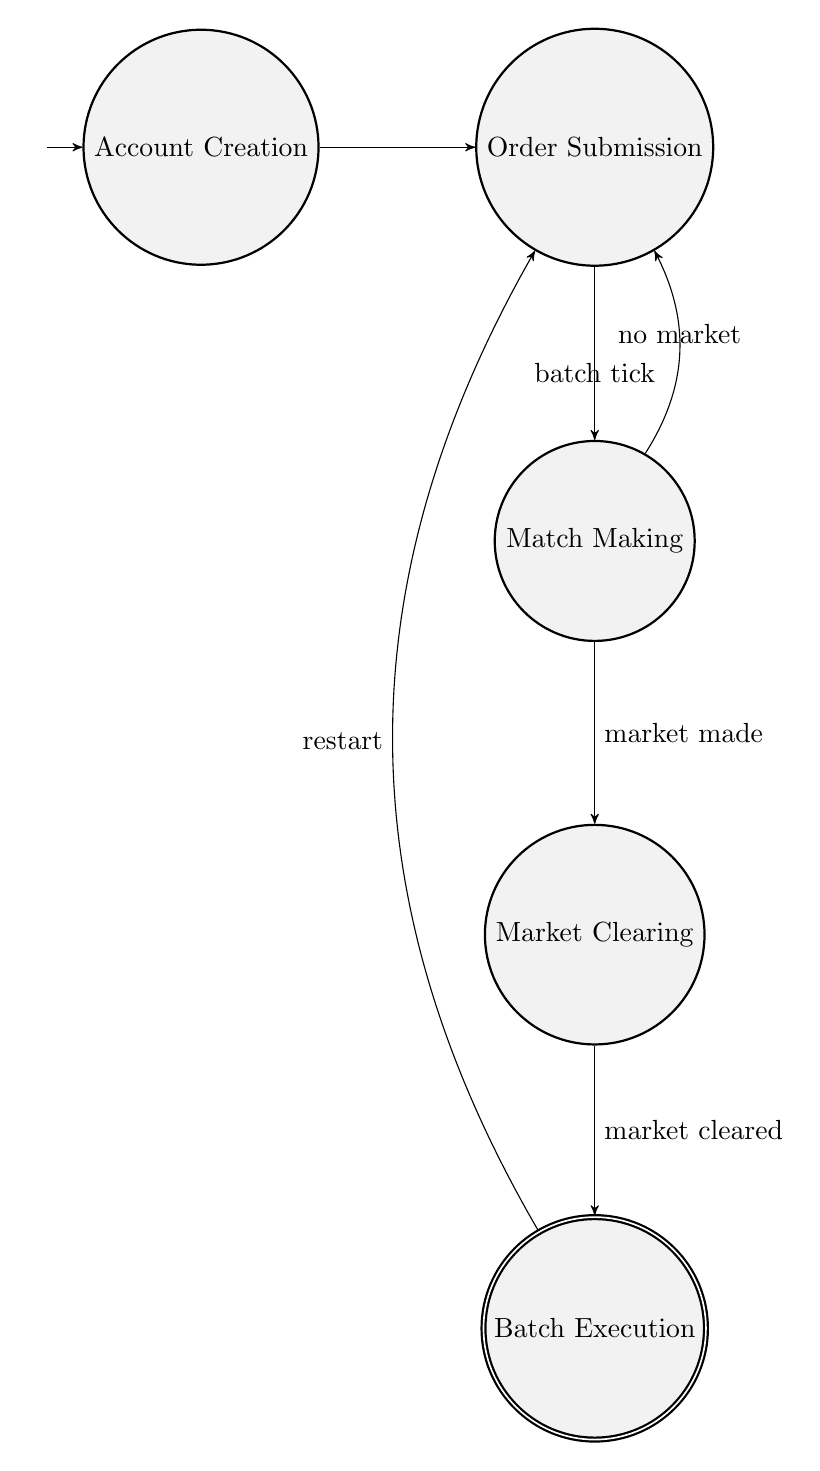
\begin{tikzpicture}[node distance=5cm,on grid,auto]
    \node[initial, state] (s0) {Account Creation};
    \node[state, right of=s0] (s1) {Order Submission};
    \node[state, below of=s1] (s2) {Match Making};
    \node[state, below of=s2] (s3) {Market Clearing};
    \node[state, accepting, below of=s3] (s4) {Batch Execution};

    \draw (s0) edge[right] node{} (s1)
          (s1) edge[below] node{batch tick} (s2)
          (s2) edge[bend right, above] node{no market} (s1)
          (s2) edge[right] node{market made} (s3)
          (s3) edge[right] node{market cleared} (s4)
          (s4) edge[bend left] node{restart} (s1);
\end{tikzpicture}

\caption{Auction State Machine}

\end{figure}


\begin{center}
    \textbf{Marketplace Auctioneer}
\end{center}

We assume the existence of a \emph{non-trusted} auctioneer $\Lambda$ that
publishes a master auctioneer key $A_{auction}$ ahead of time. The auction
itself is uniquely identified by $A_{auction}$ from the perspective of the
system due to the \emph{Shadow Chain} qualities of the system. The auctioneer
implements a non-custodial auction via \texttt{Marketplace Accounts} which use
a new unique key derived from $A_{auction}$ as the second public key in the
2-of-2 multi-sig. The auctioneer accepts and validates orders off-chain, aides
an agent in modifying their account before expiration, proposes a valid batch
to each of the agents matched in an instance of the auction, and produces a
batch execution transaction which modifies accounts appropriately, and creates
a series of corresponding channel leases.

\begin{center}
    \textbf{Account Creation}
\end{center}

Before being able to participate in the marketplace, we require that an agent
first create a \texttt{Marketplace Account}. A \texttt{Marketplace Account} is
a non-custodial account that forces an agent to commit capital in the form of
Bitcoin to the market for a period of time. As we require agents to fully back
all orders within an account, we eliminate a number of order spoofing vectors.
Additionally, the time-locked non-custodial nature of the account ensures a user
is able to recover their funds fully without any additional on-chain
transactions (aside from the sweeping transaction).

\begin{center}
    \textbf{Marketplace Order Units}
\end{center}

We abstract over the base satoshi unit and define a \texttt{unit} from the PoV
of the marketplace which is the base unit in which all orders are expressed and
settled in. We assume that the value of a given \texttt{unit} is set such that
even a single lease of the smallest unit is still economical from the
perspective of the base blockchain and on-chain fees. All orders \emph{must} be
divisible by a whole unit, and the final clearing volume of a given batch is
also expressed in units.

\begin{center}
    \textbf{Order Submission}
\end{center}

Once an agent has created a valid \texttt{Marketplace Account}, they can enter
the order submission phase. It's important to note that this order submission
takes place \emph{off-chain}. Only the final execution of an auction batch
takes place on-chain. During the order submission phase, agents are free to
modify their accounts and orders. Only valid orders will be accepted to be
eligible for the next auction iteration.

\begin{center}
    \textbf{Market Clearing}
\end{center}

Every $\Upsilon$ minutes, the auctioneer attempts to \emph{clear} the marketplace.
An auction can be cleared if the lines of supply and demand cross such that at
least a single unit is bought/sold. As the market has no explicit closing time,
it's possible that during a market epoch, no market can be made. In the
scenario that a market can be made, then rather than each participant pay what
they bid, the auctioneer instead uses a single clearing price based on the
market's clearing price algorithm.

\begin{center}
    \textbf{Batch Execution}
\end{center}

Once a market has been cleared, we enter the batch execution phase. During this
phase, the auctioneer sends a batch proposal $\Pi$, which describes the
proposed market clearing structure. $\Pi$ may either be a plaintext description
of a valid clearing solution, or a more "argument" describing one.  Valid
batches are then bundled into a single \texttt{Batch Execution
Transaction} that updates all involved accounts, and creates any channel leases
bought/sold in the batch. After a period of time $\Upsilon$ has elapsed, the
market is restarted with any new orders and account being considered for market
clearing.

\subsection{Lightning Channel Leases}
\begin{center}
\textbf{Liquidity Maker \& Taker}
\end{center}

We begin by introducing the concept of a \texttt{Liquidity Taker}: 

\theoremstyle{definition}

\begin{definition}{(Liquidity Taker).} % call Lease instead? also define CLM earlier in the process? 
    A Liquidity Taker is an agent in a Channel Liquidity Market seeking to
    \emph{obtain} new \emph{inbound} channel liquidity of size $A_{sat}$ for a
    period of $T_{block}$ Bitcoin blocks. 
\end{definition}

A taker is prepared to either boostrap the inbound liquidity with their own
on-chain coins, or pay a \emph{premium} in order to receive a "lease" of
liquidity from another agent in the market. Takers populate the \emph{demand}
side of our market. They require new inbound liquidity in order to be able to
immediately receive payments on the network, or to better position themselves
as a routing node within the network. 

A natural companion to the Liquidity Taker agent within a \texttt{CLM} is the
\texttt{Liquidity Maker}: 

\theoremstyle{definition}
\begin{definition}{(Liquidity Maker).}

A Liquidity Taker is an agent in a Channel Liquidity Market seeking to earn
\emph{yield} by deploying up to $A_{sat}$ Bitcoin into the Lightning Network
for up to a period of $T_{block}$ Bitcoin blocks, earning a profit $\alpha$. 

\end{definition}

Notice that we utilize Bitcoin block-time rather than wall-clock time (Median Past
Time (cite)) in these definitions, as we seek to enforce these durations using
Bitcoin Script and using block-time is more objective compared to wall-clock time. 

The profit ($\alpha$) earned by a \texttt{Liquidity Maker} takes two forms: 
\begin{itemize}
   \item A one-time \emph{premium}, $R_{premium}$, commanded by the Maker which
       reflects the latent demand and time-value of regular coins vs "lifted
       coins" (coins placed in channels). 

   \item Ongoing recurring revenue, $F_c$,  in the form of forwarding fees
       earned by facilitating payments to their matched taker. 
\end{itemize} 


We argue that the existence of such Channel Liquidity Markets will increase the
\emph{efficiency} of capital deployed to a payment channel network by allowing
agents to signal the relative demand of lifted coins compared to non-lifted
coins. Additionally, such markets also allow an existing routing node on the
network to \emph{re-allocate} lifted coins from a low-velocity section of the
sub-graph, to one of higher velocity: 

\begin{theorem}[Channel velocity revenue] % remove? never used in a proof or anything 
Holding all channel liquidity equal, channels allocated to a higher velocity
section of the sub-graph will yield a higher $F_c$  than channel allocated to a
low-velocity section of the sub-graph. 
\end{theorem}

Intuitively, if each payment flow sourced at an incoming channel $C_i$ and sunk
at at outgoing channel $C_o$ pays and equal forwarding fee per flow, then for a
fixed unit of time, a higher velocity channel will result in higher total
revenue in a time slice. 

The role of Channel Liquidity Markets in a payment channel network is to reduce
information asymmetry by allowing agents to signal their preferences for lifted
coins vs non-lifted coins. The existence of \emph{venues} where these markets
can be carried out benefits the wider network by allowing agents to determine
where their liquidity if most demanded on the network. % remove?

\begin{center}
\textbf{Channel Leases}
\end{center}

With our two primary agents defined we now move on to the definition of a
Lightning Channel Lease: 

\begin{definition}{(Lightning Channel Lease).} 
    A Lightning Channel Lease is defined as, $\Gamma = \{P_{T}, P_{M}, A_{sat},
    D_{block}, r_{i} \}$, where:
\end{definition}

\begin{itemize}
    \item $P_{T}$ is the \texttt{secp256k1} public key (cite) of the
\texttt{Liquidity Taker}. 
    \item $P_{M}$ the public key for the \texttt{Liquidity Maker}. 
    \item $A_{sat}$ is the total amount of Bitcoin within the contract.
    \item $D_{block}$ is the duration of the contract expressed in Blocks.
    \item $r_{i}$ is the per-block interest rate as discovered in the $i$th
    instance of the market.
\end{itemize}

Note that the premium $R_{P}$ as referenced above is parametrized in using the
\emph{lease duration} $D_{blocks}$: $R_{P}(D_{blocks}) = r_i * D_{blocks}$ as
we deal in simple, rather than compounding, interest.  The duration of the
contract $D_{blocks}$ is of great interest as similar to U.S Treasury auctions,
a \emph{yield-curve} (cite) can be constructed based on the matched contents of
a given auction iteration. % mention t-bills


\subsection{Non-Custodial Auction Accounts}

In order to participate in the auction, we require all participants to deposit their
trading balance into a Marketplace Account:

\theoremstyle{definition}
\begin{definition}{(Marketplace Account).}
A marketplace account is a \emph{non-custodial} account defined as, $\Psi =
\{K_{sat}, T_{blocks}, P_{acct}, \Omega_{nodes} \}$ where.
\end{definition}

\begin{itemize}
    \item $K_{sat}$ is the total amount of Bitcoin available within the account.
    \item $T_{blocks}$ is the absolute expiry height of the account. 
    \item $P_{acct}$ is a \texttt{secp256k1} public key  that \emph{uniqely} identifies the account.
    \item $\Omega_{nodes}$ is a set of Lighting Network nodes controlled by the account.
\end{itemize}

We stress that these accounts are \emph{non-custodial} in that after a period
of time $T_{blocks}$ the agent is able to freely remove the funds from their
account. Before this period has passed, an agent may require the aide of the
auctioneer to close, deposit, or withdraw funds from their account. In the case
of the \texttt{Liquidity Taker}, the funds within the account $K_{sat}$, must
be enough to pay for any desired premium. Conversely for the \texttt{Liquidity
Maker}, we require all funds they wish to lease out to be deposited into the
account. 

This structure, which forces all participants to fully commit all funds they
wish to use within the marketplace into a non-custodial account, is similar to
the concept of Fidelity Bonds (cite). This structure has a number of desirable
properties including:

\begin{itemize} % what else? 
    \item \textbf{Order spoofing mitigation}: Within the CLM, as all orders
        must be "fully backed", it isn't possible to place a "fake" order that
        cannot be filled.

    \item \textbf{Time value opportunity cost}: By forcing all agents to
        suspend funds they wish to use within the market, those funds cannot be
        used elsewhere, thereby adding an implicit cost to joining the
        marketplace. 

    \item \textbf{Deterministic batch execution construction}: As we'll see in
        later sections, the existence of a fixed account for each agent
        simplified the clearing and execution process within the auction
        lifecycle. 

\end{itemize}

These accounts in the abstract may take many forms, but as we focus on Bitcoin,
as detailed in later sections, these accounts will take the form of a multi-sig
output, with one key belonging to the auctioneer. 

% define other operations for Deposit(), Withdraw(), Renew(), Close() or leave to the section below 

\subsection{Order Structure \& Verification}

With our channel lease contract and account structure defined, we now move on
to our order structure. As with any auction, orders are how the agents express
their \emph{preferences} with respect to what they wish to buy and sell.
Importantly, all orders within the market must be backed by a valid non-expired
account, and must carry an \emph{authentication tag} which prevents order
spoofing, and also ensure proper integrity of a given order once it has been
submitted.

\begin{center}
\textbf{Order Structure}
\end{center}

We define an \texttt{Order} within the context of a \texttt{CLM} as follows: 

\theoremstyle{definition}
\begin{definition}{(Order).}
    An \texttt{Order} is a authenticated $n$-tuple: \\ $\Theta = \{O_{type}, K_{nonce},
    V_{ver}, P_{acct}, \Delta_{base}, \Delta_{aux}, T_{auth} \} $, where:

\end{definition}

\begin{itemize}
    \item $O_{type} \in \{\texttt{Ask}, \texttt{Bid}\}$ denotes if an order is
        an Ask or a Bid. In addition to the version, this may affect how the
        $\Delta_{aux}$ attribute is parsed.

    \item $K_{nonce}$ is an \emph{order nonce} which uniquely identifies this
        order, and is typically derived as $K_{nonce} = \sample
        \mathbb{Z}_{p}$.

    \item $V_{ver}$ is the \emph{version} of this order. As we'll see below,
        the version used as an upgrade mechanism, and is needed in order to
        parse any newly added fields, as well as compute the digest required to
        check the authentication tag attached to an order.

    \item $P_{acct}$ is the public key that uniquely identifies this account. 

    \item The set of base order details is: \\ $\Delta_{base} = \{
        \alpha_{rate}, A_{sat}, M_{pub}, L_{pub}, A_{addr}, C_{type},
    D_{blocks}, F_{chain} \}$, where:

    \begin{itemize}

        \item $\alpha_{rate}$ is the desired \emph{per-block} rate that the owner
            of the order wishes to buy/sell a channel lease at. Further below, this
            may be referred to as the \texttt{BPY} or block percentage yield.

        \item $A_{sat}$ is the total contract size expressed in lease \emph{units}.
            Restricting orders to whole units simplifies preference matching within
            the system.

        \item $M_{pub}$ is the multi-sig public key to be used when creating
            the funding output (cite) of the tranction. % abstract out more?

        \item $L_{pub}$ is the identity public key (cite) of the Lightning
            Node that wishes to buy/sell this channel.

        \item $A_{addr}$ is the network address to be used to connect to the
            backing $L_{pub}$ to initiate the channel funding process if this
            order is matched. % too low level for this portion?

        \item $C_{type}$ is the \emph{type} of channel to be created if this
            order is matched.

        \item $D_{blocks}$ is the target \emph{lease duration} of the contract.

        \item $F_{chain_{max}}$ is the max chain fee expressed in $sat/byte$ that
            the own of said order is willing to pay within a batch.

    \end{itemize}

    \item The set of \emph{auxillary} details is implcitily defined by the
        order version $V_{ver}$.

    \item $T_{auth}$ is an authentication tag that allows the auctioneer, and
        other traders to validate the integrity and authenticity of the order.


\end{itemize}

An order allows a \texttt{Liquidity Taker} or a \texttt{Liquidity Maker} to
express their \emph{preference} with respect to what type of channel lease
they're looking to buy/sell.

\begin{center}
\textbf{Order Validation}
\end{center}

Returning back to our tag $T_{auth}$, we will now specify how such a tag is to
be computed, and verified. In the abstract, we require that the tagging scheme
is \seufcma \enspace secure (cite). Given this security requirement, we define
two polynomial-time algorithms: (\texttt{GenOrderTag}, \texttt{VerifyOrderTag})
with the following requirements:

\begin{itemize}
    \item \texttt{GenOrderTag($P_{acct_{priv}}$,$\Theta$)} $\rightarrow$ $T_{auth}$.
        Given an input of the private key that corresponds to the public key of
        an account, and the complete order details, a valid tag $T_{auth}$ is
        generated.

    \item \texttt{VerifyOrderTag($P_{acct}$,$\Theta$, $T_{auth}$)} $\rightarrow$ $b$.
        Given a public key of an account holder, a valid tag, and the order
        itself, \texttt{VerifyOrderTag} outputs $b=1$ if the tag is valid.
\end{itemize}

As we use a public-key based tagging technique, the validity of an order is
verifiable by any other active trader within the marketplace including the
auctioneer of the market place.


\subsection{Auction Design}

In this section, we describe the abstract definition of a \texttt{Channel
Liquidity Marketplace}, which addresses each of the issues presented in the
bootstrapping section of the background, by creating a new form of batched
auction which allows \texttt{Liquidity Takers} and \texttt{Liquidity Makers}
to buy/sell Lightning Channel Leases in a non-custodial manner.

\subsubsection{Auction Specification}

In this section, we'll now specify the behavior and requirements of an using abstract
\texttt{Channel Liquidity Marketplace} instance. We define the expected
behavior and the client-facing interface of a \texttt{CLM} instance. A
\texttt{CLM} is a tuple of polynomial-time algorithms divided into five
distinct but related categories:
\begin{itemize}
    \item System Initialization: \texttt{SystemInit}
    \item Account Operations: (\texttt{NewAccount}, \texttt{ModifyAccount})
    \item Order Book Maintenance: (\texttt{SubmitOrder}, \texttt{CancelOrder})
    \item Market Clearing: (\texttt{MatchMake}, \texttt{MarketClearingPrice}, \texttt{ClearMarket})
    \item Batch Execution: (\texttt{ConstructBatch}, \texttt{ExecuteBatch})
\end{itemize}


With behavior and semantics as expressed below. \\

\begin{center}
    \textbf{System Initialization}
\end{center}

Before the market place can be used, we require it to be initialized by the
auctioneer. This initialization is a one-time process, and doesn't result in
any trapdoor or "toxic waste" material being produced: \\

\texttt{SystemInit($1^{\lambda}, \Upsilon_{min}$)} $\rightarrow$ ($P_{auction_p}$,
$P_{auction_s}, \Psi_{A}$). Denoting the security parameter as $\lambda$, the
    \texttt{SystemInit} algorithm takes as input the security parameter, and
    the batch interval $\Upsilon_{min}$ expressed in minutes, and outputs a
    public ($P_{auction_p}$) and private ($P_{auction_s}$) key pair for the
    auctioneer. The auctioneer's public key will be used as an parameter in
    algorithms related to account creation, modification, and batch execution.
    This algorithm also returns $\Psi_{A}$, which is a special account owned by
    the auctioneer that will be used to collect fees, and during batch
    construction.

\begin{center}
    \textbf{Account Operations}
\end{center}

In order to create an account, agents will need to interact with the auctioneer
itself. After account creation an account can freely be modified (close,
deposit, withdraw, etc) if the account isn't part of an active batch: \\

\texttt{NewAccount($1^{\lambda}, P_{auction_p}$)} $\rightarrow$ $\Psi$. The
\texttt{NewAccount} algorithm takes as input our security parameter, and the
auctioneer's public key, and outputs a new account for the new agent within the
marketplace. We require that all resulting accounts within the marketplace be
\emph{unique}. We permit a single logical agent to have multiple accounts. \\

\texttt{ModifyAccount($\Psi, P_{auction_p}$)} $\rightarrow$ ($b, \Psi^\prime$).
The \texttt{ModifyAccount} algorithm takes an existing valid account $\Psi$ and
the auctioneer's public key and performs an account modification. The algorithm
returns $b=1$ if the modification was successfully, and $b=0$ otherwise. An
account modification may fail if the target account is already part of a
pending batch. An account modification can either:
\begin{itemize}
    \item Deposit new coins into the account.
    \item Withdraw coins from the account.
    \item Close the account by removing all coins from the account.
\end{itemize}

Note that as each of these operations require an on-chain transaction, they can
freely be batched with other on-chain transactions, or even the transaction
that executes an auction's batch.

\begin{center}
    \textbf{Order Book Maintenance}
\end{center}

Once accounts in the marketplace are open, agents are able to submit orders
between batch epochs. The \emph{size} of all orders is expressed in units, and
as we mention below, we permit partial matches of an order. A partial match can
either update the order state in place, or require the agent to re-submit a new
valid tag for the modified order in the batch execution phase: \\

\texttt{SubmitOrder($\Theta, T_{auth}$)} $\rightarrow$ $b$. The
\texttt{SubmitOrder} algorithm takes as input a structurally sound order
$\Theta$, and its authentication tag $T_{auth}$ and outputs a bit $b$. The bit
$b=1$ if the order is valid according to market place rules, and the
\texttt{VerifyOrderTag} returns $b=1$ given the specified parameters. \\

\texttt{CancelOrder($\Theta, K_{nonce}^\prime$)} $\rightarrow$ $b$. The
\texttt{CancelOrder} given an existing order $\Theta$ and the \emph{opening} of
the $K_{nonce}$ commitment $K_{nonce}^\prime$ and returns $b=1$ if the
commitment opening is valid, and there exists an order identified by the base
$K_{nonce}$ value.

\begin{center}
    \textbf{Market Clearing}
\end{center}

Once all orders have been placed, and the batch interval of $\Upsilon$ has
elapsed, the auctioneer will attempt to clear the market using the following
algorithms: \\

\texttt{MatchMake($\{\Theta_0, \ldots, \Theta_n\}$)} $\rightarrow$
$\Phi_b = \{(\Theta_{b_0}, \Theta_{a_0}), \cdots, (\Theta_{b_n}, \Theta_{a_n})\}$. The
\texttt{MatchMake} algorithm takes as input the set of valid orders submitted
during the past batch interval and outputs a series of tuples which reflect
properly matched orders matched orders. $\Theta_a$ represents an order whose
$O_{type} = \texttt{Ask}$, while $\Theta_b$ represents an order whose $O_{type}
= \texttt{Bid}$. Note that since we allow \emph{partial} matches, a given order
may appear multiple times in the final match set. We require that a valid
implementation be able to perform proper \emph{multi-attribute} (cite) matching
due to the existence of the $\Delta_{aux}$ portion of an order's structure. \\

% state the specified constraints as a linear program??

 
\texttt{MarketClearingPrice($\Phi_b$)} $\rightarrow$ $c_{price}$. The
\texttt{MarketClearingPrice} algorithm accepts the set of orders matched by the
\texttt{MatchMake} algorithm and returns the \emph{market clearing price} of
the prior batch. The precise market clearing price algorithm is left as a free
parameter, with algorithms such as first-rejected-bid (cite) or
last-accepted-bid (cite) likely being used. Utilizing of a single market
clearing price is intended to promote fairness (cite) (all traders pay the same
price!).  \\

% give example of FRB and/or LAB here? 

% iamge of LAB clearing price here? 

\texttt{ClearMarket($\Psi_{A}, \Phi_b, \{\Psi_0, \dots, \Psi_n\}, c_{price}$)}
$\rightarrow$ $(\Psi_{A}^\prime, \{\Gamma_0, \dots, \Gamma_n\},
\{\Psi_{0}^\prime, \dots, \Psi_{n}^\prime\})$. The \texttt{ClearMarket}
algorithm takes as input a prior set of matched orders within a batch, the
auctioneer's account, the set of accounts involved in the bach, and the market
clearing price of a given batch and outputs: a set of channel leases to be
created by a batch and a set of updated accounts which represents the state of
the involved accounts post batch as well as an updated version of the
auctioneer's account which may have accrued any trading fees during market
clearing.

% cdots, ldots, or just dots -- need to make sure consistent everywhere

\begin{itemize}
    \item As shorthand, we use $\Delta_i$ to refer to a cleared batch (the set of
            resulting accounts after the updates have been made to produce the
            set of desired channel leases).
\end{itemize}

% takes the set of matched orders, and accounts, creates set of new accounts
% (diffs) 

\begin{center}
    \textbf{Batch Execution}
\end{center}

Once we've been able to make a market, and have the description of the
resulting market state (the accounts, and the channel leases to be created), we
can now move on to \emph{executing} the resulting batch. We use the following
algorithms to do so:  \\ 

\texttt{ConstructBatch($\Delta_i$)} $\rightarrow$ $B_{t_i}$. The
\texttt{ConstructBatch} algorithm takes a valid market clearing (which can be
seen as a delta on the auction state) and returns a valid transaction, which
\emph{atomically} executes the given batch on the blockchain. \\

\texttt{ExecuteBatch($B_{t_i}$)} $\rightarrow$ $b=$. The \texttt{ExecuteBatch}
algorithm takes a fully valid batch and attempts to commit it, by confirming
the transaction in the target base blockchain. Once the batch has been
confirmed, all operations contained within a batch are considered executed, and
can be used as inputs to additional iterations of the auction life cycle.

% have it return the batch ID? batch ID not shown any where there?

% have auction attribute section enumerating all from the blog post spill over
% portion?


\iffalse
shadow chain section: 
  * define as state machine that returns tate, then later define state in specific section to the the input of all the utxos and other state 
  
 ShadowChain:
    * Init() -> lambda params, w/e w/e 
    * state = InitState(auctioneerUtxo)
    * state = stateStep(state, stateDelta) -- a qurom needed to state step, 
    * propose set of updates to all 
        * for account := range accounts {
            proopse state 
         }
     * state_i = UpgradeState(state_i) 
     * state = {operatorKey, k_1, .., k_n}
     * state = stateFunc(state, proposal, executionEnv)
          * env can change off-chain, no need to on-chain upgrades, identified by hash/identifier 
     * order of execution func as way to impl soft-forks?  
     * state = coasalce(state_,1, ..., state_n) (transaction cut thru)
     * quorum = propose(masterKey, accounts) 
     * ^ then state func 
\fi

\section{The Shadowchain: A Bitcoin Overlay Application Framework}

In this section, we present the concept of a \texttt{Shadowchain}, a
non-custodial application overlay framework that we'll use to construct a
concrete instantiation of a \texttt{CLM}. We note that shadowchains may also be
of independent interest, as they're a novel way to layer more complex
interactions on top of the base Bitcoin blockchain. We note that shadowchains
as we present them can be implemented on the base Bitcoin blockchain today
without any additional changes or enhancements. However, further extensions to
Bticoin such as non-interactive signature aggregation (cite) and covenants
(cite) can serve to dramatically increase the scalability traits of a
shadowchain.

\subsection{High-Level Description}

First, we provide a high-level description of the shadowchain application
framework. 

\textbf{The Shadowchain Usecase}. A shadowchain can be used to implement
non-custodial smart contract systems on top of the base Bitcoin blockchain.
Typically one would opt for a shadowchain if the complexity of the state
transition logic of the smart counteract system cannot be fully expressed using
the base Bitcoin Script.  Shadowchains allow an application designer to use the
Bitcoin blockchain for what it's best for: censorship resistant settlement,
pushing the more complex portions of the application (state, logic, etc)
\emph{off-chain}.

\textbf{Shadowchain Roles \& Lifted UTXOs}. A shadowchain has two primary
classes of agents: users, and the orchestrator.  The orchestrator defines the
state transition function of the shadowchain, a set of non-trusted
initialization parameters, and upgrade mechanisms. A user is able to join a
shadowchain by "lifting" their UTXOs \emph{into} the higher-level shadowchain.
The process of lifting (defined further below) entails the user placing funds
within a time-lock released multi-sig output between itself and the shadowchain
orchestrator. 

\textbf{Shadowchain Operation}. The shadowchain orchestrator accepts
transaction data from users, then periodically proposes a new \emph{shadowchain
block}. A shadowchain block takes as input the set of \texttt{Lifted UTXO}s
which accepted the latest block proposals, and produces a set of \emph{new}
UTXOs, which are the end state after the state transition function has been
evaluated. A shadowchain is even permitted to use \emph{multiple} distinct state
transition functions. As the funds of an end user cannot move without both
multi-sig signatures, users are able to fully validate (possibly using
techniques such as zero knowledge proofs (cite shafi)) that the
resulting UTXO state was properly derived from the known state transition
function.  Note that due to this structure complex "exit-games", or fraud
proofs are not required as as a user simply won't sign off on a fraudulent
state, and a user's UTXO is always manifested (in a base form) on the main
blockchain.

\textbf{Ephemeral Lifted UTXOs}. In the scenario that the shadowchain orchestrator
disappears, or is unresponsive, users are able convert their lifted UTXO into a
regular one, by spending their coins after the time-lock has expired. This
construct of an \emph{ephemeral} lifted UTXO has a number of desirable properties
on the application level, as the time-locked commitment of funds can serve
to mitigate a number of application-level issues such as spam or sybil
resistance.

\textbf{Shadowchain Cut-Through} As the evolution of a state transition
function happens \emph{off-chain}, it's possible to coalesce several distinct
shadowchain blocks into a single block which is the composition of the
successive invocations of the state transition function. This technique is
similar to transaction cut-through (cite), but performed in a multi-party
setting. Leveraging this technique, the shadowchain orchestrator can optimistically
treat the current latest shadowchain transaction in the mempool as an in-memory
data structure to be updated off-chain (via transaction replacement techniques
(cite)), with the state being "written to disk" once confirmed. As a result,
it's possible to commit several shadowchain states (possibly hundreds) in a
single logical Bitcoin transaction.

\textbf{Shadowchain Upgrades}. Finally, similar to the base blockchain, a
shadowchain can also be \emph{upgrade} in a forwards and backwards compatible
manner. In other words, it's possible for a shadowchain orchestrator to
\emph{soft-fork} the state transition logic by restricting a valid state
transition to enable new behavior. Notably, the operator can do this in a
de-synchronized manner as only those wishing to use features in the new state
transition function need to adhere to the new rules. Additionally, an operator
can opt to also introduces new backwards incompatible state transition functions.
Due to the inherent batched nature of Bitcoin transaction, an operator can
commit multiple logical shadowchain blocks (with distinct state transition
functions) in a single atomic Bitcoin transaction.

To summarize, the shadowchain application framework is a novel technique for
constructing overlay applications on the base Bitcoin chain in a non-custodial
manner. Shadowchains avoid the complexity of fraud proofs and exit-games by
ensuring that the user has custody of their funds at all times and is able to
fully validate any proposed state transition. Shadowchains are able to compress
several logical state transitions into a single Bitcoin transaction using a
multi-party cut-through technique. An orchestrator of a shadowchain is also
able to upgrade the state transition logic on the fly, in a purely off-chain
manner.


\subsection{Comparison To Related Frameworks}

% do later?

\subsection{The Shadowchain Framework}

In this section, we present the abstract shadowchain application framework.
Applications are intended to use this framework, providing implementations of
specified virtual functions to fully specify and execute their application.

\subsubsection{Shadowchain Orchestrator}

First, we introduce the glue that keeps a shadowchain together, the
orchestrator:

\theoremstyle{definition}
\begin{definition}{(Orchestrator).} The \texttt{Orchestrator} is a non-trusted
    entity at the root of a shadowchain, parametrized by its long-term public
    key: $O_{chain} = P_{O}$. The duty of an \texttt{Orchestrator} is to
    propose new blocks (the result of a state transition) to the set of live
    \texttt{Lifted UTXO}s that make up the shadowchain.
\end{definition}

A given \texttt{Orchestrator} is a non-trusted entity, and can be uniquely
identified by its longer-term public key. The long-term public key $P_{O}$ can
also be used to uniquely identify a given shadowchain, similar to the Genesis
Block hash of a normal blockchain.

\subsubsection{Lifted UTXOs}

Next, we define the \texttt{Lifted UTXO} which is the representation of a
user's state within a given shadow chain:

\begin{definition}{(Lifted UTXO).} A \texttt{Lifted UTXO} is a tuple, 
    $ \phi_{U} = (A_{sat}, T_{expiry}, P_{u}, P_{o})$, where:
\end{definition}

\begin{itemize}
    \item $A_{sat}$ is the size of an \texttt{LO} (\texttt{Lifted UTXO})
        expressed in \emph{satoshis}.

    \item $T_{expiry}$ is the \emph{absolute} expiry height of the \texttt{LO},
        after-which the owner is able to unilaterally move the funds back to
        the "base" Bitcoin blockchain.

    \item $P_{u}$ is the public key of the end-user, which is $1/2$ of the
        public keys used in the public key script of the output which manifests
        this \texttt{LO} on the base blockchain.

    \item $P_{o}$ is the public key of the \texttt{Orchestrator}, typically
        derived from its base long-term key $P_O$. This key will be used as the
        other half of the multi-sig script of the on-chain manifestation of the
        \texttt{LO}.
\end{itemize}

% actually don't use LO here after all?

The construct of a \texttt{Lifted UTXO} is similar to the existing concept of a
Fidelity Bond (cite), yet with an application specific twist. This process is
akin to creation a new 'account' within a Shadowchain. The time-lock release
nature of the UTXO means a user can always recover funds if the
\texttt{Orchestrator} becomes unresponsive. In addition to this, a natural cost
in the form of chain fees is added which increases the barrier for potentially
malicious users to interact with the shadow chain.

\subsubsection{The Shadowchain}

In this section, we present the abstract definition of a shadowchain, building
upon the definition provided above. In addition to this, we describe the
typical shadowchain life cycle using the aid of some additional helper
functions, which are also intended to be supplied by the core application logic
itself.

\begin{center}
    \textbf{Shadowchain Components}
\end{center}

First, we define the core components of the shadowchain. 

\begin{definition}{(Shadowchain).} An instantiation of a \texttt{Shadowchain}
    is defined as a tuple: $\Sigma = (U_{L}, U_{O}, \Delta_F, E_{exe},
    A_{T})$, where:
\end{definition}

\begin{itemize}
    \item $U_{L} = \{\phi_i, \cdots, \phi_n\}$ is the set of non-expired
        \texttt{Lifted UTXO}s observed by the orchestrator.

    \item $U_{0}$ is the current UTXO orchestrator, where they may accrue
        application level fees.

    \item $\Delta_F =  \{ \Delta_{f_0}, \cdots, \Delta_{f_n} \}$ is the set of
        current state transition functions.

    \item $E_{exe}$ is the abstract execution environment of the shadowchain
        which all participants will use to verify the correctness of a proposed
        state transition.

    \item $A_{T}$ is the abstract form of the structure of the higher-level
        application's fundamental transaction.

\end{itemize}

\begin{center}
    \textbf{Shadowchain Algorithms}
\end{center}

Given the above components, we define the operation of a shadowchain using a
series of polynomial-time algorithms segmented into the following logical
categories:

\begin{itemize}
    \item System Initialization: \texttt{InitChain}
    \item UTXO Management: (\texttt{LiftUTXO}, \texttt{UnliftUTXO}, \texttt{ExitChain})
    \item Block Proposal \& Validation: (\texttt{ConstructBlock}, \texttt{ProposeBlock})
    \item Chain Execution: \texttt{CommitBlock}
    \item Block Cut-Through: \texttt{CoalesceBlocks}
    \item Chain Upgrade: \texttt{UpgradeChain}
\end{itemize}


With behavior and semantics as expressed below. \\

\begin{center}
    \textbf{System Initialization}
\end{center}

Before a shadowchain can be used for a given application, it is required that
the system be initialized to obtain the long-term public key of the auctioneer,
as well as the execution environment, and set of state transition functions: \\

\texttt{InitChain($1^{\lambda}$)} $\rightarrow$ $(U_{0}, P_{0}, \Delta_F,
E_{exe})$. Given the security parameter $\lambda$ (expressed in unary), the
\texttt{InitChain} method returns the initial self-lifted UTXO of the
orchestrator, the long-term public key of the orchestrator, and the set of
initial state transition functions along with the starting execution
environment.

% need to define the function signature ok

\begin{center}
    \textbf{UTXO Management}
\end{center}

Once the chain has been initialized, given the parameters of the shadowchain,
users can being lifting their UTXO to be able to participate in shadowchain
blocks and operations. The process of entering the shadowchain is referred to as
UTXO Lifting, while exiting is the reverse process: \\

\texttt{LiftUTXO($T_{expiry}, \{U_{N_0}, \ldots, U_{N_n}\}, P_{0}$)}
$\rightarrow$ $\phi_{U}$. The \texttt{LiftUTXO} algorithm takes a series of
normal UTXOs ($U_N$), the absolute expiration height of the UTXO, and the
long-term public key of the Orchestrator $P_{0}$ and outputs a new
\texttt{Lifted UTXO} for the target user. The sum of the set of input UTXOs
must be greater-than-or-equal to the size of the resulting \texttt{Lifted
UTXO}. \\

\texttt{ExitChain($\phi_{U}, B_{height}$)} $\rightarrow$ $U_{N}$. Given a lifted
UTXO with expiration height $T_{expiry} > B_{height}$, where $B_{height}$, the
\texttt{ExitChain} method spends an existing lifted UTXO and resolves the
user's funds in a regular unencumbered UTXO. Users will use this algorithm if
they wish to exit the chain, with the Operator no longer being responsive. \\ 

\texttt{UnliftUTXO($\phi_{U}$)} $\rightarrow$ $U_{N}$. Given a lifted UTXO the
\texttt{UnliftUTXO} method create a new normal un-lifted UTXO output
which returns all funds to the user. This is the optimistic version of the
\texttt{ExitChain} algorithm, in that it requires cooperation from the
orchestrator as the time-release clause of the Lifted UTXO's script is not yet
unlocked.

% add section for transaction submission?

\begin{center}
    \textbf{Block Proposal \& Validation}
\end{center}

Once a shadowchain has a sufficient number of lifted UTXOs, and the system has
been fully initialized, block proposal and validation can commence. This
process is similar to the process of nodes broadcasting transactions, and
miners ordering them within blocks in the base Bitcoin system: \\

% set of lifted utxos, set of transactions, exe env, state transition funcs
\texttt{ConstructBlock($\phi_{live}, T_{xn}, E_{exe}, \Delta_F$)} $\rightarrow$
$B_S$. Given inputs of the set of 'live' Lifted UTXOs, the set of transaction
belonging to the live UTXOs, the execution environment, and the current set of
valid state transition
functions, the \texttt{ConstructBlock} outputs a valid shadowchain block to
extend the current machine chain. Where: 
\begin{itemize}
    \item $\phi_{live} = live(\{\phi_{U_0}, \cdots, \phi_{U_N}\}$ is the set of
            'live' Lifted UTXOs where the $live$ algorithm uses a heart-beat
            like protocol to detect the current set of active users.

    \item $T_{xn}$ is the application-specific transaction format used within
        the shadowchain.

    \item $B_S = (T_{xn}, \{\phi_{U_0}, \cdots, \phi_{U_N}\}, \Delta_{f},
        \{\phi_{U_0}^\prime, \cdots, \phi_{U_N}^\prime\}, U_{A})$, is the
        shadowchain block itself, which is composed of the set of application
        transaction, input Lifted UTXOs, the resulting output UTXOs after
        applying the set of state transition functions, and $U_{A}$ any new
        application-specific UTXOs produced as a result of the state transition
        function.
\end{itemize}

Once a block has been constructed, the operator of the shadowchain now must
propose said block to the set of live Lifted UTXOs before we can move onto the
next phase of shadowchain operation. As a given user may reject a block, either
implicitly due to being offline, or explicitly due to a violation of the
shadowchain consensus rules, then this phase may be repeated a number of times.
The operator will use the following algorithm to propose blocks: \\

\texttt{ProposeBlock($B_S, \phi_{live}$)} $\rightarrow$ $b$. The
\texttt{ProposeBlock} attempts to propose the given shadowchain block to the
set of live Lifted UTXOs. The algorithm returns $b=1$ if all of the
participants accept the block. Once all participants have accepted the block,
we can now proceed to the execution and block commitment phase.

% need to add ValidteBlock for the end user

\begin{center}
    \textbf{Chain Execution}
\end{center}

Once the operator has esatblshed a stable set of participants which accept the
proposed shadowchain block, it can execute the block and commit it in the base Bitcoin blockchain: \\

\texttt{CommitBlock($B_S$)} $\rightarrow$ $(b, TX_{id})$. The
\texttt{CommitBlock} takes a valid shadowchain block, and attempts to obtain
all necessary witnesses to unlock the Lifted UTXOs to re-create them post state
function application along with any new application-specific UTXOs. The
algorithm returns $b=1$ if the operator was able to succesfully obtain all
necessary witnesses, and brodcast the Bitcoin transaction which commits the
shadowchain block. Otherwise, the operator may need to re-propose a new block
to a sub-set of the live Lifted UTXOs.

\begin{center}
    \textbf{Block Cut-Through}
\end{center}

Given the sturcutre of a shadowchain block, and the state transition function
itself, it's possible for a shadowchain operator to compress several distinct
shadowchain blocks into a single instance that is equivalent to the succesive
state transtion function application on each distinct shadowchain block: \\

\texttt{CoalesceBlocks($\{B_{S_0}, \cdots, B_{S_N}\}$)} $\rightarrow$
$B_{S}^\prime$. Given a series of \emph{consecutive} shadowchain blocks, the
\texttt{CoalesceBlocks} algorithms compresses each consecutive block into a
single block $B_{S_N}$ which has an equivalent output state to the serial
appliation of the state transition functino on each individual shadowchain
block. \\

The \texttt{CoalesceBlocks} algorithm is similar to the concept of transaction
cut-through (cite) for UTXO-based blockchains. Using this algorithm, the
operator is able to propose a new equivalent block which produces the same set
of net Lifted UTXO outputs, along with any other application specific outputs
produced by any of the intermediate blocks. This can be done post-facto, and
also in an optimsitic manner in order to coalesce several unconfirmed
shadowchain blocks into a single one.

% diagram for cut thru

% re-phrase using function composition?

% add a real algorithm that details the process of it

\begin{center}
    \textbf{Chain Upgrade}
\end{center}

The process of upgrading the chain in terms of the \emph{types} of
application-level transactions offered, or the set of valid state transition
functions can be done entirely off-chain in a de-synchronized manner. In order to
update the environment, state transition functions, or the applicatoin-level
transactions, the operator simply needs to utilize the following algorithm: \\

\texttt{UpgradeChain($\Delta_{new}, E_{exe}^\prime, T_{xn}^\prime$)}
$\rightarrow$ $\bot$. The \texttt{UpgradeChain} is an algorithm that's executed
entirely in an off-chain manner, than lets the operator of the shadowchain
upgrade some or all of: the application transaction data, the execution
environment, and the set of state transition functions. Due to the nature of
the shadowchain, in order to utilize this new functionality each user must
update their local state. However, note that the Lifted UTXO remains the same,
as the operator's long-term public key hasn't changed.

\subsubsection{Shadowchain Operation}

In this section, we'll put together the above algorithms to outline the main
execution loop of the shadowchain from the perspective of the operator as well
as participants. Shadowchain operation can be viewed as a linear deterministic
state machine that uses the main Bitcoin blockchain in order to transition to
certain states.

% insert shadowchain diagram here

\begin{center}
    \textbf{Operator State Machine}
\end{center}

The main Operator State Machine loop first attempts to process any new UTXO
lifting requests, then will optimistically attempt to merge in any existing
unconfirmed shadowchain blocks that can be coalesced. Independent of either of
these clauses, we'll then enter into our main loop where the operator attempts
to construct a new block given the set of live transaction, propose the block
to the set of live UTXOs, filter out any participants that rejected the block,
before finally attempting to commit the new block within the chain.

%\procedureblock[syntaxhighlight=auto]{OrchestrateChain(utxos, env, funcs)}{
%    until \neg s
%}
        % run loop
        % process account lifting
        % try to coaclse any blocks
        % construct block
        % propose block 
        % take those that accept then construct block with
        % commit block

\begin{pchstack}[boxed,center, space=1em]
    \procedure[linenumbering, syntaxhighlight=auto]{\texttt{OrchestrateChain($\Delta_{F}, E_{exe}$)}}{
        repeat \\
        \t if \texttt{haveNewLiftReqs()} \\
        \t \t \{\phi_{new}\} \gets \texttt{liftNewUTXOs($P_{O}$)} \\
        \t \t \{\phi_{U}\} \gets \phi_{U} \cup \phi_{new} \\
        \t if \texttt{numUnconfBlocks()}>1 \\
        \t \t B_{S}^\prime \gets \texttt{CoalesceBlocks(unconfBlocks())} \\
        \t \t (b, txid) \gets \texttt{CommitBlock($B_{S}^\prime$)} \\
        \t T_{xn} \gets \texttt{liveTransactions()} \\
        \t \phi_{live} \gets \texttt{liveLiftedUTxos()} \\
        \t b \gets 0 \\
        \t while b==0 \& len(\phi_{live}) > 0 \\
        \t \t B_{S} \gets \texttt{ConstructBlock($\phi_{live}, T_{xn}, E_{exe}, \Delta_{F}$)} \\
        \t \t b \gets \texttt{ProposeBlock($\phi_{live}, B_{S}$)} \\
        \t \t if b== 0 \\
        \t \t \t \phi_{live} \gets \texttt{filterRejects($\phi_{live}$)} \\
        \t \t if b==1 \\
        \t \t \t (b^\prime, TX_{id}) \gets \texttt{CommitBlock($B_{S}$)} \\
     }

     \procedure [linenumbering, mode=text ]{ Oracle $O$}{
         some code \\
         more code
     }
\end{pchstack}


\begin{center}
    \textbf{Participant State Machine}
\end{center}

The main state machine if each shadowchain participant is essentially a mirror
of the orchestrator state machine. First we'll process any requests to modify
our existing Lifted UTXO, gather up any unconfirmed transactions, then await a
new block proposal by the orchestrator.

\begin{pchstack}[boxed,center, space=1em]
    \procedure[linenumbering, syntaxhighlight=auto, addkeywords={await}]{\texttt{ExtendChain($\phi_{U}, \Delta_{F}, E_{exe}$)}}{
        repeat \\
        \t T_{xn}^\prime \gets \texttt{unconfTxns()} \\ 
        \t \texttt{submitTxns($T_{xn}$)} \\ 
        \t B_{S}^\prime \gets await \quad \texttt{recvBlockProposal()} \\
        \t b \gets \texttt{ValidateBlock($B_{S}^\prime$)} \\
        \t if b == 1 \\
        \t \t \texttt{sendWitnesses($U_{O}$)} \\ 
        \t\t b^\prime \gets await \quad \texttt{blockFinalize} \\
        \t\t if b^\prime == 1 \\
        \t\t \t \texttt{localCommitBlock()}
     }

     \procedure [linenumbering, mode=text ]{ Oracle $O$}{
         some code \\
         more code
     }
 \end{pchstack}

% lift utxo if non empty
% read off txn queue, submit operation to operator
% wait for proposal
% validate proposal, accept
% sign for lifted utxo accept block
% go to top


\section{Lightning Pool: A Channel Liquidity Marketplace as a Shadow Chain}

In this section, we build upon the prior sections outlining the abstract
\texttt{Channel Lease Marketplace} definition, as well as shadowchain
operation, and construct out \textbf{Lightning Pool} implementation at a
low-level. We first being by detailing our implementation of the \texttt{CLM}
algorithms, as well as our choice of certain free parameters. With this
concrete structure in place, we'll then go up a layer of abstraction to
demonstrate how Lightning Pool can be operated as a shadowchain on Bitcoin
today, without any further modifications enhancements.

\subsection{Instantiating a CLM}

\subsubsection{System Initialization}

\begin{center}
    \textbf{Batch Key Parameter}
\end{center}

Before an instance of Lightning Pool can be used by willing agents, the system
must first be initialized. This operation can be performed only by by the
Orchestrator of the auctioneer. Within the system, we'll utilize incremented
Elliptic Curve point which we refer to as the \texttt{batchID} for several
operations. The \texttt{batchID} serves to uniquely identified a given batch,
and is incremented after each successful batch. \\

The \texttt{batchID} itself is a nothing up my sleeve (NUMs) point which has
been generated in a manner that no one, not even the auctioneer knows the
discrete log to. The raw serialized \texttt{batchID} (for the very first batch)
within the \textbf{Lightning Pool} system can be expressed in the following
syntax (displayed using hex-encoding of a compressed key encoding of the batch
key itself): \\
\[
    B_{k_0} = NUMS_{gen}(1^\lambda)
\] \\

Let the current \textbf{batchID} for the $n^{\text{th}}$ batch be $B_{k_i}$.
Let $G$ be a cyclic group of order $N=pq$, generated by an element $g$.  We now
define two helper functions to allow us to "seek" round the \textbf{batchID}
key-space:
\begin{pcvstack}[boxed,center, space=1em]
     \begin{pchstack}
        \procedure[linenumbering, syntaxhighlight=auto]{\texttt{IncrementBatchKey($B_{k_i}$)}}{
            return B_{k_i} + g
         }

         \procedure[linenumbering, syntaxhighlight=auto]{\texttt{DecrementBatchKey($B_{k_i}$)}}{
            return B_{k_i} - g
         }
     \end{pchstack}

     \begin{center}
     \procedure[linenumbering, syntaxhighlight=auto]{\texttt{InitBatchKey}}{
        return B_{k_0}
     }
     \end{center}
\end{pcvstack} % lol kinda overkill here?, also fix the above formal EC definitions

With the system initializtion , we'll now move onto specifying the structure of
a \texttt{Marketplace Account} within \textbf{Lightning Pool}.

\begin{center}
    \textbf{Auctioneer State Initialization}
\end{center}

Now that we have defined the set of initialization and manipulation methods for
our batch key parameter, we'll move onto the initialization of the remaining
system. In order to prevent key-reuse across the entire system, we employ a
similar key-derivation scheme to that of the Lightning Network's current
commitment transaction format (cite). This key derivation will be used within
all account scripts within the system, as well as the auctioneer's main
account. \\

First, we define a helper function for deriving the auctioneer's current key
parameterized by the current \texttt{batchID}. As noted above, the
\texttt{batchID} serves as both a public key within the system as well as a
counter. The \texttt{batchID} may be expressed as a normal compressed public
key, or as an integer $N_{b}$ which denotes the scalar multiple off-set from
the starting batch key $B_{k_0}$: $[B_{k_0}]N_{b}$. We define the
\texttt{auctioneerScript} as follows: 

\begin{pcvstack}[boxed,center, space=1em]
    \procedure[linenumbering, syntaxhighlight=auto]{\texttt{auctioneerScript($A_{pk}, B_{k_i}$)}}{
        A_{pk_i} \gets A_{pk} + H(A_{pk} \concat B_{k_i}) \\
        return \texttt{OP\_CHECKSIG $A_{pk_i}$}
    }
\end{pcvstack} 

The script itself is a simple script that simply verifies a proper auctioneer
signature given a particular \texttt{batchID}. In order to make all scripts
uniform (as the account scripts are \texttt{P2WSH} outputs, we wrap this script
in a \texttt{P2WSH} layer of indirection as well. With this algorithm defined,
we can now define the \texttt{SystemInit} implementation for \textbf{Lightning
Pool} that derives the first batch key along with the starting script of the
auctioneer. \\

\begin{pcvstack}[boxed,center, space=1em]
    \procedure[linenumbering, syntaxhighlight=auto]{\texttt{SystemInit($1^{\lambda}, \Upsilon_{min}$)}}{
        batchKey \gets \texttt{InitBatchKey()} \\
        A_{sk} \sample \mathbb{Z}_{p} \\
        A_{pk} \gets G A_{sk} \\
        aScript \gets \texttt{auctioneerScript($A_{pk}$, batchKey)}\\ 
        pkScript \gets \texttt{p2wsh(aScript)} \\ 
        return (A_{sk}, A_{pk}, \texttt{utxo(pkScript, seedSats)})
     }
\end{pcvstack} 

Once the third return value, auctioneer's master account has been confirmed.
Participants are able to open accounts, submit orders, and finally participate
in auction batches.


\subsubsection{Lightning Pool Accounts}

Next, we move onto the \texttt{Marketplace Account} structure for agents within
the \texttt{Lightning Pool} marketplace itself. Similar to the auctioneer's
master account, we apply a key derivation scheme that combines the auctioneer's
key, the batch key, a key supplied by the trader, and a distinct trader
specific secret to ensure, that: 
\begin{itemize}
    \item A \texttt{P2WSH} output script is \emph{never} re-used.
    \item Traders rotate keys with each batch.
    \item The set of trader keys using within a batch itself is
        indistinguishable w.r.t the input keys referenced and newly created
        outputs keys.
\end{itemize}

Let $P_{t}$ be a trader's base key, $S_{t} \sample \mathbb{Z}_{p}$ be an
account-specific secret generated by the trader, and $P_{A}$ be the
auctioneer's long-term public key.We define a new algorithm
\texttt{traderAccountScript} which will be used to derive the \texttt{pkScript}
for a given trader:

\begin{pcvstack}[boxed,center, space=1em]
    \procedure[linenumbering, syntaxhighlight=auto]{\texttt{traderAcctScript($P_{t}, S_{t}, P_{A}, B_{k_i}$)}}{
        t \gets H(B_{k_i} \concat S_{t} \concat P_{t}) \\
        P_{t}^\prime \gets P_{t} + (t * G) \\
        P_{A}^\prime \gets P_{A} + H(P_{t}^\prime \concat P_{A}) * G \\
        \texttt{witnessScript} \gets \{ \\
            \t P_{t}^\prime \enspace \texttt{OP\_CHECKSIGVERIFY} \\
            \t P_{A}^\prime \enspace \texttt{OP\_CHECKSIG} \\
            \t \texttt{OP\_IFDUP} \\
            \t \texttt{OP\_NOTIF} \\
            \t \t T_{blocks} \enspace \texttt{OP\_CHECKLOCKTIMEVERIFY} \\
            \t \texttt{OP\_ENDIF} \\
        \} \\
        return \texttt{witnessScript}
     }
\end{pcvstack} 

% make sure to double check the above!

The above script can either be spent via the time out clause using the
following witness stack, using \texttt{nil} value passes an empty signature to
force execution of the timeout clause.
\begin{verbatim}
nil traderSig witnessScript
\end{verbatim}

Or via the normal spend path way which will be used to authorized batches,
account closing, and any other account modifications:
\begin{verbatim}
auctioneerSig traderSig witnessScript
\end{verbatim}

Note that each trader starts using the current batch key at the time they
joined the marketplace. However, as we'll see below in the execution section, a
trader's key gets rotated with each batch they participate in, meaning that the
set of batch keys used within a trader's account output script will eventually
become de-synchronized across the market unless all trader's participate in all
batches, which is unlikely. \\

Given the \texttt{traderAccountScript} algorithm, we'll now define our
implementation of the set of \texttt{Account Operations} methods:
% missing params like amt as well, etc
\begin{pcvstack}[boxed,center,space=1em]
    \procedure[linenumbering, syntaxhighlight=auto, addkeywords={await}]{\texttt{NewAccount($1^{\lambda}, P_{auction_p}$)}}{
        k_{t} \sample \mathbb{Z}_{p} \\
        P_{t} \gets k_{t} * G \\
        \texttt{acctScript} \gets \texttt{traderAcctScript($P_{t}, S_{t}, P_{A}, B_{k_i}$)} \\ 
        \texttt{accountTxn} \gets \texttt{makeTxn(acctScript)} \\
        \texttt{traderSignTxn(accountTxn)}\\ 
        \texttt{broadcastTxn(accountTxn)} \\
        \Psi \gets await \quad \texttt{confirmation(accountTxn)} \\
        return \Psi
     }

     \procedure[linenumbering, syntaxhighlight=auto, addkeywords={await, readInput, match, not}]{\texttt{ModifyAccount($\Psi, P_{auction_p}$)}}{
        if \texttt{inPendingBatch($\Psi$)} \\
        \t return (0, \Psi) \\ \\
        B_{k_i+1} \gets \texttt{IncrementBatchKey($\Psi, B_{k_i}$)} \\
        \texttt{acctScript} \gets \texttt{traderAcctScript($P_{t}, S_{t}, P_{A}, B_{k_i+1}$)} \\ \\
        txInputs \gets readInput \enspace \texttt{clientStream} \\
        txOutputs \gets readInput \enspace \texttt{clientStream} \\ 
        \texttt{action} = \bot \\
        match: \\
        \t \t \texttt{acctScript} \enspace not in txOutputs: \\
        \t \t \t \texttt{action} = \texttt{CLOSE} \\
        \t \t txOutputs.acctOutput.Value > \Psi.Value: \\
        \t \t \t \texttt{action} = \texttt{DEPOSIT} \\
        \t \t txOutputs.acctOutput.Value < \Psi.Value: \\
        \t \t \t \texttt{action} = \texttt{WITHDRAW} \\ \\
        \texttt{accountTxn} \gets \texttt{makeTxn(acctScript, action, txInputs, txOutputs)} \\
        \texttt{traderSignTxn(accounTxn)} \\  
        \texttt{broadcastTxn(accounTxn)} \\ \\
        \Psi^\prime \gets await \enspace \texttt{confirmation(accounTxn)} \\ 
        return \Psi^\prime
     }
\end{pcvstack} 

Notice how the \texttt{batchKey} is incremented for all account modification
operations. In this manner, the \texttt{batchKey} also serves as a sequence
number within the scripts to ensure that no scripts are re-used within the
system. 

Users are able to recover their accounts themselves if data has been lost by
scanning the chain for the above instances of \texttt{newAcctScript} and
utilizing the timeout clause within the account script of a trader's account.

% also mention account recovery?
% also need to specify the batchkey and the rest above as well?

\subsubsection{Channel Leases in the Lightning Network}

Now that we have our concrete account structure, we'll move on to presenting a
concrete instantiation of a Channel Lease based on today's widely used payment
channel implementation within Lightning Network. \\

\begin{center}
    \textbf{Channel Lease Duration Enforcement}
\end{center}

The unique component that sets apart a regular channel from one that was
created via a channel lease contract is \emph{duration} enforcement. As a
channel lease contracts states the capital must be committed to the network for
a minimum period of time, in order to implement this in a trust-minimized
manner, we must enhance the existing channel format (cite) used in the
Lightning Network today. Our tool of choice for creating minimum duration
enforced channels is the \texttt{OP\_CHECKLOCKTIMEVERIFY} (cite) op-code.
Minimally, we need to enforce the following conditions:
\begin{itemize}
    \item The \texttt{Liquidity Maker} involved in a channel lease cannot sweep
        the funds in their settled commitment output as manifested on their
        commitment or the commitment of the remote party until $D_{block}$
        Bitcoin blocks has passed since the creation of the channel lease.
    \item The \texttt{Liquidity Maker} also cannot fully sweep any funds that
        are suspended within HTLC outputs until $D_{block}$ Bitcoin blocks has
        passed.
\end{itemize}

The second item is of great importance to ensure that the seller of a channel
lease can't just move all the committed funds into HTLCs, then close the
channel and be fully refunded, netting the lease premium in the process.
Instead, we need to ensure that the node is able to resolve any HTLCs on-chain
if needed, while still being forced to commit the funds in ancestors of the
multi-sig funding output, until the lease duration has expired. \\

We now make a small modification first to the settled local output of the
\texttt{Liquidity Maker}:
\begin{center}
    \begin{verbatim}
    OP_IF
        <revoke key> 
    OP_ELSE
        <lease duration in blocks>
        OP_CHECKLOCKTIMEVERIFY
        OP_DROP
     
        <delay in blocks>
        OP_CHECKSEQUENCEVERIFY
        OP_DROP
        
        <delay key> 
    OP_ENDIF

    OP_CHECKSIG
    \end{verbatim} 
\end{center}

Next, we make a similar modification to the settled remote output of the
\texttt{Liquidity Maker}, assuming anchor output based channels (cite) are
used: 
\begin{center}
    \begin{verbatim}
    <localKey> OP_CHECKSIGVERIFY
    <lease duration> OP_CHECKLOCKTIMEVERIFY
    1 OP_CHECKSEQUENCEVERIFY
    \end{verbatim} 
\end{center}

Finally, we modify the offered HTLC outputs of the \texttt{Liquidity Maker} for
their local commitment transaction:
\begin{center}
    \begin{verbatim}
     OP_IF
        <revoke key> 
    OP_ELSE
        <lease duration in blocks>
        OP_CHECKLOCKTIMEVERIFY
        OP_DROP
     
        <delay in blocks>
        OP_CHECKSEQUENCEVERIFY
        OP_DROP
        
        <delay key> 
    OP_ENDIF

    OP_CHECKSIG
    \end{verbatim} 
\end{center}

% ^ make these into funcs instead

A less trust-minimized version of channel lease duration enforcement is
possible simply by having the \texttt{Liquidity Taker} refuse a cooperative
channel closure until the lease duration has expired. With this non-script
based enforcement, the only direct option the \texttt{Liquidity Maker} has is
to \emph{force-close} their channel. However, the operator of an auction venue
can request additional information along-side orders before batch execution (as
detailed below) to identify premature force closes on-chain in order to
penalize the renegading party.

% also need to handle the remote script as well?

\begin{center}
    \textbf{Channel Lease Funding Protocol}
\end{center}

Given the existence of a new modified chanenl $C_{L}$ that supports the channel
lease protocol, we require a new way to fund the channels as a channel
lease itself will \emph{partially-bind} the following paramters of a given
channel:
\begin{itemize}
    \item The size of the channel itself.
    \item The two multi-sig scripts used within the channel.
    \item The duration of the channel lease itself.
\end{itemize}

Rather than modifying the base funding protocol of the Lightning Network, we've
opted to instead provide a \emph{new} "side-loadable" partial funding binding
API we call a channel shim (cite). A channel shim allows a party $A$ to
\emph{expect} certain parameters of the channel itself. Given the
\texttt{pendingChanID} which is used to identify an unfinalized channel within
the Lightinng Network (cite), an algorithm \texttt{RegisterChannelShim($\Gamma,
P_{a}$, outPoint)} instructs a Lightning Node to use a \emph{prearranged} public key as
specified within channel lease $\Gamma$ for its portion of the multi-sig output
used within the ultimate channel.

The existence of the channel shim API allows a node to proceed in the set up of
a channel for which it may not yet know the \emph{full} funding transaction to.
Given the lease, and the expected outpoint, both sides can fully sign the
commitment transaction in a manner that doesn't incur any risk as due to the
account structure, they'll need to sign off on the batch funding transaction
itself before it can be broadcast.

The funding flow using this new order shim, assuming that match making and
market clearing has already occurred, resembles the following flow, with Alice
being the \texttt{Liquidity Taker} and Bob being the \texttt{Liquidity Maker}:
\begin{pcvstack}[boxed,center,space=1em]
    \procedure{\texttt{leaseInit}}{
        (\Gamma, \texttt{leasePoint}) \gets B_{t_i}.\texttt{lease[Alice \concat Bob]} \\
        P_{a} \gets \Gamma.P_{T} \\
        P_{b} \gets \Gamma.P_{M} \\
        \texttt{RegisterChannelShim($\Gamma, P_{a}$, leasePoint)}
    }

    \procedure{\texttt{ChannelShimFundChannel}}{
        \textbf{Alice} \> \> \> \textbf{Bob} \\
        \texttt{leaseInit()<++>} \\
        \> \sendmessage{<-}{top=\texttt{OpenChannel($P_b$)}} \> \\
        \> \sendmessage{->}{top=\texttt{AcceptChannel($P_a$)}} \> \\ 
        \> \sendmessage{<-}{top=\texttt{FundingCreated(leasePoint)}} \> \\
        \> \sendmessage{->}{top=\texttt{FundingSigned}} \> \\ 
    }
\end{pcvstack} 

In this modified flow, notice that the taker returns the \emph{pre-generated}
public key to use within the multi-sig within the \texttt{AcceptChannel}
method, and the taker uses the canned \texttt{leasePoint} as the input to the
funding transaction. As we'll see below the \texttt{leasePoint} itself is
generated after market clearing, and during the construction of the batch
execution transaction. The \texttt{leasePoint} as it exists on the batch
execution transaction creates a new channel point that staifies the details of
the negotiated channel lease $\Gamma$: the amount of the leaase, and the
pkSCript of the two multi-sig keys $P_a$ and $P_b$.

We note that the channel shim abstraction has a number of indepneddent uses
including strong layer isolation for more elaborate multi-party channel
protocols. Notice how the base \textbf{BOLT} funding flow is unmodified,
meaning that a higher level application can handle the specified details of the
multi-party transaction protocol, while the unmodified Lightning node software
manages the underlying channel itself.

\subsubsection{Order Structure}

With our concrete account structure and channel lease semantics in place, we'll
now outline the precise structure of orders as implemented in \textbf{Lightning
Pool}. As a \texttt{CLM} is a \emph{sealed-bid} auction, the set of active
orders within an auction epoch isn't known to a given participant within the
auction. Instead, bids are submitted directly to the auctioneer, and may
optionally be cancelled between batch epochs as well. Using the fundamental
\texttt{unit} notion for expressing the \emph{quantity} of an order, we permit
partial matching in addition to specifying a \emph{minumum} matchable amount by
adding a new field $M_{match}$ to an order within the $\Delta_{aux}$ set of
additional order attributes.

% orders
% order verification w/ the tag, EUF-CMA
% mention min node tier as aux, batch fee rate as aux

\begin{center}
    \textbf{Order Tag Generation \& Validation}
\end{center}

Next, we specifying order tag generation and validation. Before verifying an
order, the order $\Theta$ itself is serialized in order to generate the message
digest of the order.  This is done by concatenating each item of the order
into a single byte stream, with the set of $\Delta_{aux}$ attributes specifying
a custom serialization mechanism. 

For our tag generation, we opt to utilize an \seufcma \enspace signature scheme. As we
target the base Bitcoin blockchain, \texttt{Lightning Pool} utilizes Schnorr
signatures implemented over the \texttt{secp256k1} elliptic curve. In addition
to having the trader that submits an order sign the order message digest, we
also require that all the backing Lightning nodes of the order also include a
signature as well.  As the number of backing nodes for a given account may be
numerous, rather than accepting individual signatures for each node, we instead
require the account operator and all backing nodes to present a \emph{single}
Schnorr signature. As we also want have our order tagging scheme be secure
against key rogue-key attacks (cite), we select the \texttt{MuSig}
multi-signature scheme. \\

Given the \texttt{MuSig} multi-signature scheme, we define the following
algorithms used in our order tagging scheme:
\begin{itemize}
    \item Let \texttt{Sign($\{P_{0}, \dots, P_{i}\}, M$)} $\rightarrow$
        $\sigma$, be an algorithm that returns a valid \texttt{MuSig}
        multi-signature signed by the set of public keys on message $M$.

    \item Let \texttt{Verify($\{P_{0}, \dots, P_{i}\}, \sigma, M$)}
        $\rightarrow$ $b$ be an algorithm that returns $b=1$ if the passed
        signature is a valid \texttt{MuSig} multi-signature signed by the set
        of public keys for the message $M$. 
\end{itemize}

Given these algorithms, we now define our order tag generation and validation
implementations:

\begin{pcvstack}[boxed,center, space=1em]
    \procedure[syntaxhighlight=auto]{GenOrderTag($P_{acct}$, $\Theta$)}{
        m \gets K_{nonce} \| V_{ver} \| P_{acct} \| \Delta_{base} \concat \Delta_{aux} \\
        tag \gets \texttt{Sign$(\{\Theta.L_{pub}, \Theta.M_{pub}\dots \}, m$)} \\
        return tag
    }

    \procedure[syntaxhighlight=auto]{VerifyOrderTag($P_{acct}$, $\Theta$)}{
        m \gets K_{nonce} \| V_{ver} \| P_{acct} \| \Delta_{base} \concat \Delta_{aux} \\
        b \gets \texttt{Verify($\{P_{acct}, P_{M_pub_0}, \dots, P_{M_pub_i} \}, m$)} \\
        return b
    }
\end{pcvstack}

We omit the implementations of \texttt{SubmitOrder} and \texttt{CancelOrder} as
the depend on the specific environment in which the auctioneer is implemented
in. We only add that the pre-image to an order nonce $K_{nonce}^\prime$ is
known only to the agent that places the order. As we touch on within the future
direction section, this commitment structure also has a number of independent
uses outside of order cancellation.

\subsubsection{Node Rating Agencies}

Recalling the set of initial requirements that were set our in section 4, it's
critical that Lightning Pool reduces information symmetry for the buyer by
allowing them to gauge the quality of the node selling a channel lease before
they enter into an agreement. In order to achieve this, we introduce the
concept of a Node Rating Agency. An rating's agency will allow the buyer of a
lease to either query the agency in an ad-hoc manner, or specify that they only
wish to be matched with nodes that reside on a certain \emph{tier}. \\


Let $\hat{T_{node}} = \{\hat{t_0}, \dots, \hat{t_n} \}$ be the set of possible
ratings that can be given to a Lightning Node with $\hat{t_0}$ containing
\emph{all} known Lightning Nodes, and $|\hat{t_i}| > |\hat{t_{i+1}}| \enspace
\forall \enspace i < n$, where $n$ is the number of available tiers. In other
words, we create a series of node sets, with the higher node tiers having less
nodes than lower tiers.  This creates a natural system of concentric circles
where as the tier index increases, the set of nodes shrinks, and eventually
only higher quality nodes remain. \\

Building off this notion of tiered node sets, we define the following algorithm
for our node rating agency:
\begin{pchstack}[boxed,center, space=1em]
    \procedure[syntaxhighlight=auto, addkeywords={map}]{NodeTier($L_{pub}$)}{
        \texttt{nodeMap} \gets map(\hat{T_{node}}) \\
        t_{node} = \texttt{nodeMap[$L_{pub}$]} \\
        return t_{node}
    }
\end{pchstack}

Given this algorithm, we now specify our of the additional auxiliary order
attribute $\Delta_{aux}$ as: \[
    (N_{tier}, \dots) = \Delta_{aux}
\]

During match making, we then require the constraint that a given bid order
$\Theta_{bid}$ will only be matched with an ask order $\Theta_{ask}$ if the
following constraint is met:
\[
    \Theta_{bid}.N_{tier} >= \texttt{NodeTier($\Theta_{ask}.L_{pub}$)}
\]

% use arg min above? 

\subsubsection{Uniform Price Market Clearing \& Matching}

With our order structure, and the notion of the Node Rating Agency outlined, we
now move on to the concrete market clearing and match making within Lightning
Pool.

\begin{center}
    \textbf{Order Matching}
\end{center}

As mentioned, due to the set of additional constraints outside of simply the
posted price and available supply, we employ a multi-attribute mach making
algorithm. Specifically we opt to utilize a greedy algorithm for the purpose of
match making, rather than attempt to find an optimal solution using
techniques such as mixed integer linear programming. In this section, we focus
primarily on the set of base attributes, leaving the consideration of a
trader's axillary attribute preferences to later work. \\

% add above don't do it since can be expensive

First, we define an abstract algorithm which will be used to determine if a
given ask order $\Theta_{ask}$ is compatible preference-wise to a given bid
order $\Theta_{bid}$:
\begin{itemize}
    \item \texttt{MatchPossible($\Theta_{bid}, \Theta_{ask}$)} $\rightarrow$
        $(b, n_{unit})$. This algorithm returns $b=1$ if the given ask and bid
        are compatible from a match making perspective. If the orders are
        compatible, then $n_{unit}$ represents the number of units that can be
        matched across the two orders.
\end{itemize}

% algo for MakeMake to queue accumulate until able to be matched

Given this function we define our implementation of the \texttt{MatchMake}
algorithm:
\begin{pchstack}[boxed,center, space=1em]
    \procedure[linenumbering,syntaxhighlight=auto, addkeywords={map, filter, sort}]{\texttt{MatchMake(O: $\{\Theta_0, \ldots, \Theta_n\}$)}}{
        \texttt{matchSet} \gets \{\} \\
        \texttt{asks} \gets sort(filter(O, \Theta_{i}.O_{type} == Ask)) \\
        \texttt{bids} \gets sort(filter(O, \Theta_{i}.O_{type} == Bid)) \\
        for bid in bids: \\
        \t for ask in asks: \\
        \t \t if \texttt{MatchPossible(bid, ask)}: \\
        \t \t \t \texttt{matchSet} = \texttt{matchSet} \cup (ask, bid) \\
        return \texttt{matchSet}
    }
\end{pchstack}

We note that several optimizations here are possible to reduce the worst-case
running time of the algorithm which we leave open for future work. We also
assume that the set of valid orders has been flittered out before being passed
into this algorithm based on the current target batch fee rate and the posted
max batch fee rate of each order.

\begin{center}
    \textbf{Uniform Price Clearing}
\end{center}

Once we've had our set of candidate matches, we'll now move on to the market
clearing phase. During the market clearing phase, two distinct operations are
carried out:
\begin{itemize}
    \item A trader's account state is updated to reflect any lease premiums
        earned due to matches, chain fees paid in the  batch execution
        transaction, fees paid to the auctioneer, and finally the debit for any
        sold channels from their account.

    \item We determine the uniform clearing price for a given potential batch.
\end{itemize}

These two actions comprise the \texttt{ClearMarket} and
\texttt{MarketClearingPrice} algorithms. For our market clearing price, we
select the Last Accepted Bid market clearing rule (cite), chosing to go with a
buery's mid marking price. Given this price clearing algorithm, we now define
our implementaion of the market clearing algorithms:
\begin{pcvstack}[boxed,center, space=1em]
    \procedure[linenumbering,syntaxhighlight=auto, addkeywords={len, filter, sort}]{\texttt{MarketClearingPrice($\Phi_b$)}}{
        \texttt{lastPair} \gets \Phi_b[len(\Phi_b - 1)] \\ 
        return \texttt{lastPair.bid.$\alpha_{rate}$}
    }

    \procedure[linenumbering,syntaxhighlight=auto, addkeywords={newLease, filter, sort}]{\texttt{ClearMarket($\Psi_{A}, \Phi_b, \{\Psi_0, \dots, \Psi_n\}, c_{price}$)}}{
        \texttt{leases} \gets \{\} \\
        \texttt{accts} \gets \{\} \\
        for \texttt{orderPair} in \Phi_b: \\
        \t \texttt{lease} \gets \texttt{newLease(orderPair)} \\
        \t \texttt{orderPair.taker.balance} \mathrel{{-}{=}} \texttt{lease.premium} \\
        \t \texttt{orderPair.maker.balance} \mathrel{{+}{=}} \texttt{lease.premium} \\ \\
        \t \texttt{orderPair.taker.balance} \mathrel{{-}{=}} \texttt{exeFee(lease.amt)} \\
        \t \texttt{orderPair.maker.balance} \mathrel{{-}{=}} \texttt{exeFee(lease.amt)} \\
        \t \texttt{$\Psi_{A}$.balance} \mathrel{{+}{=}} \texttt{exeFee(lease.amt)} \\ \\
        \t \texttt{leases} \gets \texttt{leases} \cup \texttt{lease} \\
        \t \texttt{accts[orderPair.taker]} \gets \texttt{orderPair.taker} \\
        \t \texttt{accts[orderPair.maker]} \gets \texttt{orderPair.maker} \\ \\
        return (\Psi_{A}, \texttt{leases, accts})
    }
\end{pcvstack}

Notice that we omit the observance of chain fees, as that will be applied to
each input/output during the later batch construction phase.

% matching, multi-attribute
% series of matching predicates?
% market clearing
% selection of LAB, flash some theory

\subsubsection{Auction Batch Execution}

Once we've cleared the market, we'll now move onto the batch execution phase.
During this phase, we'll construct the batch transaction which executes a given
batch, and also gather all the necessary witnesses for each participant of the
batch so we can properly spend their on-chain account outputs. Remember
that due to the non-custodial structure, a trader will fully validate a given
batch before they sign off on it.

\begin{center}
    \textbf{Batch Transaction Construction}
\end{center}

A given batch transaction contains the following inputs: the set of trader
account inputs involved in the batch, and the input of the master auctioneer
itself. In addition to these inputs which can only eb spent each each user
authorized the proposed batch, we also add the following outputs: a trader's
new incremented account output which reflects the market clearing, the set of
channels created as part of the channel lease, and the incremented auctioneer
account. Note that the format of the batch transaction itself may change
multiple times during this phase if participants reject the batch, or if fee
changes causing the auctioneer to consider a subset of the prior set of orders.

Taking this into consideration, we define our implementation of
\textbf{ConstructBatch} as follows: 
\begin{pcvstack}[boxed,center, space=1em]
    \procedure[linenumbering,syntaxhighlight=auto, addkeywords={len, newTx, sort}]{\texttt{ConstructBatch($\Delta_i$)}}{
        \texttt{tx} \gets newTx() \\
        \texttt{tx.addIn($\Delta_i.\Psi_{A}$)} \\ \\
        for acct in \Delta_i.\Psi: \\
        \t \texttt{tx.addIn(acct.prevOut)} \\
        for acct in \Delta_i.\Psi^\prime: \\
        \t \texttt{acct.Value} \mathrel{{-}{=}} \texttt{feeShare($\Delta_i$, acct)} \\
        \t \texttt{tx.addOut(acct.txOut)} \\ \\
        for lease in \Delta_i.\Gamma: \\
        \t \texttt{tx.addOut(lease.txOut)} \\ \\
        \Psi_{A}.value \mathrel{{-}{=}} \texttt{feeShare($\Delta_i, \Psi_{A}$)} \\
        \texttt{tx.addOut($\Delta_i.\Psi_{A}^\prime$)} \\
        return tx
    }
\end{pcvstack}

\begin{center}
    \textbf{Batch Transaction Execution}
\end{center}

Once the batch has been constructed, the auctioneer then needs to propose the
batch to each trader, and collect the necessary set of signatures required to
spend each trader's account input. During this execution phase, we assume that
this is the final set of traders that wish to be a part of this batch. Once the
auctioneer has all the necessary signatures to broadcast a batch, the batch
execution transaction can be broadcast, ending this auction epoch.  \\

Batch transaction execution itself is a multi-party protocol wherein the
auctioneer presents a valid auction batch to all involved parties, the parties
verify the batch, before finally signing off by resenting valid signatures of
the batch (thereby attesting to it) which are require to execute the batch by
committing it in the Bitcoin blockchain. \\

We define batch execution in the context of Lightning Pool as follows:
\begin{pcvstack}[boxed,center, space=1em]
    \procedure[syntaxhighlight=auto, addkeywords={sign, newTx, sort}]{\texttt{ExecuteBatch($B_{t_i}$)}}{
        \textbf{Trader} \> \> \textbf{Auctioneer} \\
        \> \sendmessage{<-}{top=\texttt{BatchPrepare($B_{t_i}$)}} \> \\
        b \gets \texttt{ValidateBatch($B_{t_i}$)} \\
        if b == 1: \\
        \t \texttt{leaseInit($B_{t_i}$)} \\
        \> \sendmessage{->}{top=\texttt{BatchAccept}} \> \\ 
        else: \\
        \> \sendmessage{->}{top=\texttt{BatchReject}} \> \\
        \> \> \text{abort if reject sent} \\ \\
        \> \sendmessage{<-}{top=\texttt{BatchSignBegin}} \> \\
        \t \texttt{ChannelShimFundChannel($\Gamma$)} \\
        W_i \gets \texttt{sign($\Gamma, B_{t_i}$)} \\
        \> \sendmessage{->}{top=\texttt{BatchSign($W_i$)}} \> \\ 
        \> \sendmessage{<-}{top=\texttt{BatchFinalize}} \> \\
        \> \> \texttt{broadcast($B_{t_i}$)}
    }
\end{pcvstack}

Once the auctioneer has gathered all the signatures $W_i$ from each participant
of the batch, then it can sign its own input in the batch transaction, and
broadcast the batch thereby finalizing execution. We now provide additional
insight with respect to the meaning of each of the messages sent above.
\begin{itemize}
    \item The \texttt{BatchPrepare} message kicks off batch execution and is
        used to \emph{propose} a new potential auction batch to an end user
        client. Upon receipt of this message, the client will attempt to verify
        the batch using the \texttt{ValidateBatch} algorithm. 

    \item If the batch is \emph{invalid} from the client's PoV, then a
        \texttt{BatchReject} message is sent. Upon receipt of the reject
        message the auctioneer will resume the protocol, excluding the
        rejecting client.

    \item Otherwise, the client accepts the batch after verifying its integrity
        by sending the \texttt{BatchAccept} message.

    \item In order to synchronize the creation of funding shims and the channel
        funding protocol itself, the auctioneer send the
        \texttt{BatchSignBegin} message. After sending the reject, the
        \emph{taker} will register a funding shim to ensure it's able to
        properly handle the incoming funding request in the next phase.

    \item Upon receipt of the \texttt{BatchSignBegin} message, the client then
        is ready to fund the channel, using the \texttt{leasePoint} which is
        present on the batch execution transaction $B_{t_i}$.

    \item Once the funding is complete (both sides have a valid commitment
        transaction), then the trader will sign its input to present a valid
        signature to the auctioneer, so the batch transaction can be completed.

    \item The final set for the auctioneer is to commit the new batch to disk,
        and broadcast the transaction to the Bitcoin network.
\end{itemize}

\subsubsection{Sidecar Channel Market Clearing \& Batch Execution}

As mentioned in the background section, a Channel Lease Marketplace is able to
also implement the abstract notion of a "sidecar channel". We begin by first
defining a sidecar channel as so:

\theoremstyle{definition}

\begin{definition}{(Sidecar Channel.} 
    A \texttt{Sidecar Channel} is defined as $\Sigma_c = \{A_{r}, B_{s}, C_{g},
    N_{sat_{in}}, N_{sat_{out}}\}$, where:
\end{definition}
\begin{itemize}
    \item $A_{r}$ is the \emph{receiver} of a new channel which may contain both
        inbound and outbound liquidity. This party may or may not already be a
        participant in the CLM.

    \item $B_{s}$ is the seller of a normal channel lease within the CLM, and
        holds an active trading account.

    \item $C_{g}$ is the \emph{gifter} of a sidecar channel who wishes to onboard
        $A_{r}$ to the Lightning Network. Note that $A_{r}$ may not even have any
        Bitcoin at all.

    \item $N_{sat_{in}}$ is the number of Bitcoin expressed in satoshis of the
        channel itself, which will be available as inbound channel bandwidth to
        $A_{r}$.

    \item $N_{sat_{out}}$ is the number of Bitcoin which is to be pushed (cite)
        to the receiver of the side car channel, allowing them to both send and
        receive.
\end{itemize}

At a high level, a sidecar channel allows Alice to buy a channel for Carol via
Bob. Pool implements sidecar channels by making a series of small modifications to
the normal marketplace operations. An end-to-end workflow resembles the
following:
\begin{itemize}
    \item Alice who already has an account in the CLM places an order to buy a
        channel. However, rather than specifying the public key and connection
        details of her own node, she uses Carol's information instead.

    \item During market clearing, if $N_{sat_{out}} > 0$, then Alice will pay
        an \emph{additional} amount of $N_{sat_{out}}$ satoshis directly into
        the account of Bob.

    \item During batch execution, rather than Alice registering a channel shim,
        she informs Carol to do so in an expectation step. Bob then uses the
        new $N_{sat_{out}}$ satoshis in his account to push the Bitcoin over to
        the channel he created between himself an Alice.

    \item To ensure the agreement is upheld, Carol uses a channel acceptor
        (cite) predicate to validate that the proper amount has been pushed.
\end{itemize}

Aside from the above modifications to our market clearing and batch execution,
everything else remains untouched. The end result is the ability to purchase a
channel for a 3rd party in the network in a trust-minimized manner. This new
ability is akin to being able to insert an edge in the network (a new channel)
between any two arbitrary but cooperating parties. As an example, an exchange
could use this flow to allow a client to withdraw directly into a \emph{new}
channel. 

\subsubsection{LSAT as Pool Tickets}

As an added layer against spam and resource exhaustion attacks, Lightning Pool
uses Lightning Service Authentication Tokens, or LSATs (cite) when interacting
with all users. In order to perform operations such as creating an account,
querying batch snapshots, etc, a valid LSAT is required. The auctioneer is able
to dynamically raise the price of an LSAT which is expressed in satoshis if
anomalous behavior is detected.

In addition to using LSATs to throttle or rate limit clients, the auctioneer is
also able to use them as a mechanism to offer up historical chain data for sale
to 3rd party observers (those without active trading accounts) of the system.

% talk about other LSAT stuff


\subsection{The Lightning Pool Shadowchain}

In this section, we complete the Lightning Pool system by demonstrating out its
implementation of a Channel Lease Marketplace can be implemented using our
shadowchain application overlay framework.

% auctioneer is the orcewstrator, etc fill in thos meethods now
% execution env is golang code
% define the state transition function: takes in orders and updates all other state likely use funcs from above

\subsubsection{Lightning Pool Accounts as Lifted UTXOs}

First, we link the concept of our non-custodial accounts in the CLM realm to a
lifted UTXO. The process of lifting and unlifting a UTXO is simply a series of
operations required to create, modify or close an account:

\begin{pcvstack}[boxed,center, space=1em]
    \procedure[linenumbering,syntaxhighlight=auto, addkeywords={map, filter}]{\texttt{LiftUTXO($T_{expiry}, \{U_{N_0}, \ldots, U_{N_n}\}, P_{0}$)}}{
        \texttt{inputs} \gets \{U_{N_0}, \ldots, U_{N_n}\} \\
        return \texttt{NewAccount($T_{expiry}, P_{0}$, inputs)}
    }

    \procedure[linenumbering,syntaxhighlight=auto, addkeywords={map, filter}]{\texttt{UnliftUTXO($\Psi_{U}$)}}{
        (b, _) \gets \texttt{ModifyAccount($\Psi_{U}, P_{auction_p}$)} \\
        return b
    }

    \procedure[linenumbering,syntaxhighlight=auto, addkeywords={map, filter}]{\texttt{ExitChain($\phi_{U}, B_{height}$)}}{
        if \phi_{U}.T_{blocks} < B_{height}: \\
        \t return 0 \\
        (b, _) \gets \texttt{ModifyAccount($\Psi_{U}, P_{auction_p}$)} \\
        return b
    }
\end{pcvstack}

Note that it's also possible to upgrade Lifted UTXOs as implemented within
Pool, as a given user is able to use the latest features in Bitcoin script to
achieve the same functionality. However, due to privacy implications, it may be
preferred to have all account scripts, and further all scripts within a batch
execution transaction be uniform.

\subsubsection{Auction Batch Proposal}

Next, we move unto patch proposal and acceptance. An auction batch within a CLM
maps 1:1 to the concept of blocks in the shadowchain domain. Given this
insight, we now define the \texttt{ConstructBlock} and \texttt{ProposeBlock}
algorithms:

\begin{pchstack}[boxed,center, space=1em]
    \procedure[syntaxhighlight=auto, addkeywords={map, filter}]{\texttt{ConstructBlock($\phi_{live}, T_{xn}, E_{exe}, \Delta_F$)}}{
        \Phi_b \gets \texttt{MatchMake($T_{xn}$)} \\
        c_{price} \gets \texttt{MarketClearingPrice($\Phi_{b}$)} \\
        \texttt{ClearMarket} \gets \Delta_F \\
        \Delta_i \gets \texttt{ClearMarket($\Psi_{A}, \Phi_{b}, \Psi, c_{price}$)} \\
        return \Delta_i
    }

    \procedure[syntaxhighlight=auto, addkeywords={map, filter}]{\texttt{ProposeBlock($B_S, \phi_{live}$)}}{
        b \gets \texttt{ValidateBatch($B_S, \phi_{live}$)} \\
        return b
    }
\end{pchstack}

The process of constructing a new block walks through each of the phases within
the auction itself. Note that a block in our system can only be constructed if
there exist a valid market clearing given the set of orders
( application-specific transactions). The auctioneer then proposes the block to
each party within the \texttt{BatchPrepare} message. Traders are then free to
accept or reject a given block. 

% need to define validate batch as well, also cast above?

\subsubsection{Shadowchain Batch Execution}

Now that we're able to lift/unlift UTXOs and propose blocks within our
Shadowchain, we now define the series of methods that will be utilized to allow
clients to execute the their local version of the state transition function to
accept new proposed batches:
\begin{pchstack}[boxed,center, space=1em]
    \procedure[linenumbering,syntaxhighlight=auto, addkeywords={map, filter}]{\texttt{CommitBlock($B_S$)}}{
        (b, TX_{id}) \gets \texttt{ExecuteBatch($B_S$)} \\
        return b
    }
\end{pchstack}

The \texttt{ExecuteBatch} algorithm does most of the heavy lifting here. Note
that if for whatever reason, execution fails, then $b=0$ is returned, and we
resume our normal state machine execution loop. At the end of the
\texttt{CommitBlock} algorithm all participants have the latest block (as they
need to be given thee block in order to sign off on it), and the block is
broadcast to the Bitcoin blockchain. After this phase, it's possible to
continue committing new blocks without waiting for prior blocks to confirm. Due
to this flexibility, the Orchestrator of the Lightning Pool shadow chain is
then able to \emph{optimistically} perform transaction cut-through to combine
several logical blocks into a single Bitcoin transaction.

% fill in the rests of the algos

\subsubsection{Unconfirmed Batch Cut-Through}

Recall that a shadowchain block can also be optimistically aggregated into a
single block. In the domain of the Lightning Pool shadowchain, combining blocks
requires ensuring that all produced channel leases will still exist in the
final combined blocks, and the end state of each account remelts any
consecutive market clearing opportunities:

\begin{pchstack}[boxed,center, space=1em]
    \procedure[linenumbering,syntaxhighlight=auto, addkeywords={set, filter}]{\texttt{CoalesceBlocks(F: $\{B_{S_0}, \cdots, B_{S_N}\}$)}}{
        \texttt{inputs} \gets set(F) \\
        \texttt{leases} \gets \texttt{extractLeases(F)} \\
        \texttt{accts} \gets \texttt{endAcctState(F)} \\ \\
        \texttt{tx} \gets \texttt{ConstructBatch($\Delta_i$(inputs, leases, accts))} \\
        b \gets ExecuteBatch(t) \\
        return b
    }
\end{pchstack}

For brevity, we omit the referenced internal algorithms, however the naming is
intended to be intuitive. Given a series of blocks $F$, we need to extract all
thee inputs referenced in each block (the series of accounts), extract the set
of all leases created within the block, and also the ending account state of
all accounts involved in the prior blocks. Note that one account may
participate in all or some of the prior blocks. The process of block
cut-through allows us to only manifest the \emph{ending state} of their account
and elide the intermediate states from the PoV of the blockchain. With these
summaries constructed, the auctioneer then construct a new batch, and executes
it using the normal algorithms.

Scalability gains are had by only manifesting the final state of each account,
as well as removing the need to manifest all intermediate transaction within
the blockchain.  All participants have an incentive to participate in this
optimistic block cut-through as they'll also end up paying less chain fees as
they only need to pay for their account input+output, and any leases created
\emph{once}. If any of the intermediate blocks confirm instead of the
cut-through block, then the process can be repeated with the new set of
unconfirmed blocks.

\subsubsection{Auction Upgrades}

Finally, we define the process by which we upgrade the CLM shadowchain itself.
As this is an off-chain process, each participant of the shadowchain is able to
execute the \texttt{UpgradeChain} algorithm simply by updating their end client
software. In addition to this we utilize two upgrade extension points:
\begin{itemize}
    \item The version of a given order.
    \item The \texttt{batchVersion} sent within the \texttt{BatchPrepare}
        message.
\end{itemize}

The version in each order allows us to add new order types over time which
implement new match making related preference expression, or brand new channel
types. The version sent along during batch execution allows us to modify
attributes such as the fee sharing scheme, or the structure of the batch
execution transaction itself.

\section{Security Analysis}

Similar to Lightning Loop, the Lightning Pool backend server is may be closed
source, but clients are able to fully verify and audit each phase of the
auction. At a high level, Pool can be seen as a “shadow chain” anchored in the
base Bitcoin blockchain. The shadow chain validates modifications to a subset
of the UTXO set (the Pool accounts) with the auctioneer acting as a block
proposer to extend the chain. State transitions are validated and accepted by
those that are involved in a new block (the auction batch). Newer clients are
even able to audit the prior history of the system in order to ensure proper
operation. Pool uses the Bitcoin blockchain for what it’s best for: global
censorship resistant batch execution.

Leveraging this shadow chain structure, users remain in control of their funds
at all times, and will only enter into agreements that they’re able to fully
verify, ensuring that channels are properly constructed and that the market is
operating as expected. Compared to existing centralized exchanges with
off-chain order execution, Pool has a number of attractive security properties:
\begin{itemize}

    \item As a non-custodial system, users are in control of their funds at all
        times.

    \item A purchased LCL will result in the creation of a channel with parameters
        that capture the preferences expressed in the initial order.

    \item If the auctioneer server is hacked, the breach doesn’t unilaterally
        compromise user funds.

    \item Orders by one trader cannot be used to spoof orders by another trader.

    \item Clients are able to verify and audit all operations carried out by the
        server during batch construction including proper order matching.

\end{itemize}


\section{Future Directions}

As is clients verify each Shadowchain blocks within the CLM system, but they
have no assurance that their order was actually included in the mach making
function. In this manner, the auctioneer can silently ignore a set of orders.
To remedy this, it is possible for tha auctioneer to publish an order
transpeacny authenticated data structure to give users a mrkle leaf receipt of
proper order inclusion.

Rather than sending over a full block, the auctioneer can instead send over a
ZKP (cite) of proper block validity. This would imporve the privacy of the
system.

As is, the maker rerecivees thier pereimum all at once. However it may bne
possible to set up another uni-directional channel in order to stream the
interest in real-time. It may further be possbile to allow others to buy/sell
the future cash flows of the "coupon channels".

\section{Related Work}

\section{Conclusion}

In this work, we've put forth a new abstraction over capital obligations in the
Lightning Network, which we call channel leases. Channel leases can be bought
and sold on a Channle Liqudiity Marketplace directly solving a series of
bootrapping challenges the network faces, commonly referred to as: the inbound
liquidity problem. To implement a Channel Lease Marketplace in a secure manner,
we put forth the concept of a shadowchain application framework which is of
independent use. We then concretely construct Lightning Pool, the first
\texttt{CLM} implemented on top of the base Bitcoin blockchain. Lightning Pool
allows those with idle capital to earn yieild on their Bitcoin, and also allows
those that need inbound to receive over the network to obtain a reliable soure
of incoming payment bandwidth.

\section{Acknowledgments}

ryan, justin, etc

\bibliographystyle{abbrv}
\bibliography{main}

\end{document}
This is never printed

